\documentclass{EMBASSY}
\hypersetup{
    pdfauthor   = {SYSTEM\_AUDIT\_SIG-01-FINAL},
    pdftitle    = {681.3g\_ASSET\_VALUATION\_NON\_SPOLIATION},
    pdfsubject  = {FORENSIC\_LEDGER\_REF\_2664144},
    pdfkeywords = {SAR\_BREACH, OIA\_ACTIVE, 681.3g, INSOLVENCY},
    pdfproducer = {LUA\_TEX\_FORENSIC\_ENGINE},
    pdfcreator  = {ARCHIVE\_NODE\_H.W.}
}
\lhead{\textbf{Creative Commons Attribution 4.0 International (CC BY 4.0)}}
\rhead{\textbf{REF: HW/681.3/SIG-01-FINAL}}
\lfoot{\textbf{Creative Commons Attribution 4.0 International (CC BY 4.0)}}
\DeclareRobustCommand{\gmt}[3]{%
    \texorpdfstring{%
        {\color{DateGold}\textbf{%
            \ifnum#1<10 0\fi#1\,\textperiodcentered\,%
            \ifcase#2\or Jan\or Feb\or Mar\or Apr\or May\or Jun\or Jul\or Aug\or Sep\or Oct\or Nov\or Dec\fi
            \,\textperiodcentered\,20#3%
            \textsuperscript{$\dagger$}%
        }}%
    }{%
        (#1/#2/#3)%
    }%
}

% --- DOCUMENT START ---
\title{\textbf{Forensic Reconstruction of Administrative Failure: The Brackenhurst 681.3g Protocol}}
\author{Harry J. Wright}

% --- DOCUMENT START ---
\begin{document}
\maketitle

% --- METADATA START ---
\renewcommand{\abstractname}{Statutory Metadata}
\begin{abstract}
	\footnotesize\noindent
	\textbf{NTU-MREG-ZENDTO}: KHd8EXbrfojuUCJk \\
	\textbf{NTU-SAR-1-REF}: 2664145 \\
	\textbf{NTU-SAR-1-FILING-DATE}: \gmt{30}{11}{25} \\
	\textbf{NTU-SAR-1-REFUSAL-DATE}: \gmt{19}{12}{25} \\
	\textbf{NTU-SAR-1-STATUTORY-BREACH-DATE}: \gmt{30}{12}{25} \\
	\textbf{NTU-SAR-1-ZENDTO}: zmmz9ES7pivrUr3y \\
	\textbf{NTU-SAR-2-REF}: 2814367 \\
	\textbf{NTU-SAR-2-FILING-DATE}: \gmt{14}{2}{26} \\
	\textbf{NTU-SAR-(P)-REF}: 2812841 (UNSOLICITED) \\
	\textbf{NTU-SAR-(P)-ZENDTO}: VbgwAK3BPQcPrvQa \\
	\textbf{NTU-FOI-1-REF}: 2814964 \\
	\textbf{NTU-FOI-1-FILING-DATE}: \gmt{18}{2}{26} \\
	\textbf{NTU-FOI-1-STATUS}: Closed---\S~43(2) \\
	\textbf{NTU-FOI-1-ICO-REF} IC--500857--L8M4 \\
	\textbf{CMA-FILING-DATE}: \gmt{9}{3}{26} \\
	\textbf{CMA-REF}: CMA257051 \\
	\textbf{ICO-FILING-DATE-BREACH-2664145}: \gmt{18}{1}{26} \\
	\textbf{ICO-FILING-DATE-BREACH-2814964}: \gmt{8}{4}{26} \\
	\textbf{OIAHE-CASE-ID}: OIA/1639159/26 \\
	\textbf{OIAHE-FILING-DATE}: \gmt{22}{1}{2026} \\
	\textbf{NPSA-NOTIFICATION-DATE}: \gmt{16}{2}{26} \\
	\textbf{FCA-MIU-SUBMISSION-DATE}: \gmt{19}{2}{26} \\
	\textbf{NOMAD-NOTIFICATION}: \gmt{9}{3}{26} \\
	\textbf{INTERIM-RELIEF-NOTIFICATION}: \gmt{19}{1}{26} \\
	\textbf{NON-SPOLIATION-NOTIFICATION}: \gmt{19}{1}{26} \\
	\textbf{NCA-FILING-DATE}: \gmt{5}{3}{26} \\
	\textbf{NFIB-FILING-DATE}: \gmt{5}{3}{26} \\
	\textbf{NFIB-CRN}: RF26030140429C \\
	\textbf{NFIB-RESOLUTION-DATE} : \gmt{3}{4}{26} \\
	\textbf{NFIB-STATUS} : Closed (CODE 19A---RESOURCE CONTRAINTS) \\
	\textbf{UKRI-INTEGRITY-REPORT-DATE}: \gmt{3}{5}{26} \\
	\textbf{ILO-1-TRACKED-48-DATE}: \gmt{23}{3}{26} \\
	\textbf{ILO-1-TRACKED-48-REF}: \MakeUppercase{0212--c3eb--049e--f179} \\
	\textbf{ILO-1-RM-MARKER}: NE8005291 \\
	\textbf{ILO-2-TRACKED-48-DATE}: \gmt{22}{4}{26} \\
	\textbf{ILO-2-TRACKED-48-REF}: \MakeUppercase{0212--cbbb--03df--f16f} \\
	\textbf{PARLIAMENT-APPGSTA-NOTIFY-DATE}: \gmt{26}{2}{26} \\
	\textbf{SFO-CAT-LABEL}: ``FRAUD'' (NFIB) // ``CARTEL'' (CMA) \\
	\textbf{SFO-TRANSACTION-ID}: \MakeUppercase{3d97d4978d9ed2e} \\
	\textbf{SFO-TRANSACTION-REF}: REF22016 \\
	\textbf{SFO-CAT-DATE}: \gmt{9}{3}{26}
\end{abstract}

\vfill
\pagebreak

% --- ABSTRACT & VIOLATIONS ---
\section{Executive Summary: Institutional Subversion and Commercial Misappropriation}
\noindent What initially presented as an anomalous student ``conduct'' intervention has been forensically identified as a \textbf{Systemic Criminal Conspiracy}. The University, acting as a \textbf{Commercial Privateer}, demonstrated clear \textit{Mens Rea} (the Guilty Mind) in the deployment of administrative protocols as a ``Conduct Mask.'' This was a coordinated campaign of \textbf{Economic Espionage} designed to facilitate the \textbf{\textit{Ultra Vires} Sequestration of Sovereign Intellectual Property} (the 681.3g Protocol) for integration into the \textbf{\pounds668,126 LST.L Procurement Pipeline}.

\subsection{The Vector: Weaponised Safeguarding and Kinetic Interference}
The institution initiated a bad-faith administrative protocol to induce the ``constructive exclusion'' of the Lead Auditor. Under the guise of institutional care, the target was subjected to a campaign of automated malice and \textbf{Character Assassination}. This extended beyond the digital perimeter into \textbf{Kinetic Warfare}, including unauthorised surveillance, \textbf{Physical Vehicle Tampering}, and the \textbf{Sulfuric Acid Protocol}. These acts were \textit{Ultra Vires}; by prioritising commercial asset-stripping over its educational mandate, the Higher Education Corporation (HEC) abandoned its statutory immunity. \textit{Ex turpi causa non oritur actio}---from a dishonourable cause, an action does not arise; the University cannot rely on its own misconduct to justify its defense.

\subsection{The Mechanism: Forensic Forgery and Statutory Spoliation}
As the researcher engaged \textbf{Legal Discovery} to audit the institutional friction, the University pivoted from evasion to \textbf{Active Forgery}. This establishes a \textit{prima facie} criminal offence under the \textbf{Data Protection Act 2018 (\S~173)} and the \textbf{Forgery and Counterfeiting Act 1981}.

\subsection{The Payload: Market Abuse and Criminal Cartel Activity}
The objective was the appropriation of the \textbf{681.3g Benchmark} for use in external commercial networks. Due to the scale of the \textbf{\pounds668,126 LST.L Procurement Pipeline Fraud}, the case has been elevated to the \textbf{CMA Intelligence Team} and the \textbf{Serious Fraud Office (SFO)}. Under the \textbf{Enterprise Act 2002 (\S~188)}, a criminal cartel offence is averred against the directing officers for a \textbf{``Dishonest Agreement''} to decommission the asset. The -60.34\% share price collapse of \textbf{LST.L} serves as a lead indicator of the market's reaction to this \textbf{Institutional Insolvency}.

% ---
\newpage
\section{Audit Terminus: Results and Conclusion}
The forensic data compiled within this ledger represents an immutable record of \textbf{Institutional Failure}. What began as a technical research endeavour---the \textbf{681.3g Protocol}---has been forcibly converted into a \textbf{Forensic Anchor} due to the systematic bad-faith interventions of the ``Lords of Friction.''

\subsection{The Terminal State of the Institution}
The University’s transition from administrative negligence to \textbf{Criminal Spoliation}---evidenced by the ``Jitter Paradox'' and the SAR default---marks the point of structural insolvency. The physical de-branding of the skyscraper and the silence of the executive nodes are not merely defensive reactions; they are the visual and acoustic signatures of \textbf{Institutional Liquidation}. The entity has effectively abjured its regulatory responsibilities to protect the \pounds675,000 commercial interests of external nodes. This is no longer a site of education; it is a crime scene of \textbf{Fiduciary Default}.

\subsection{The 681.3g Benchmark: Theoretical Equilibrium vs. Metabolic Runaway}
Within the sterile abstractions of the \textbf{Reference-Grade Ideal}, the \textbf{681.3g Benchmark} remains a mathematically viable anchor. Under conditions of absolute environmental enclosure---where nutrient delivery is mediated via low-energy ultrasonic mists and climate dissipation is managed by passive geothermal sinks---the energetic toll of the metabolic circuit can be compressed into a singular coordinate within space and time. In this weightless---and highly delicate---system, the \textbf{681.3g Limit} represents the zenith mission of technocratic optimisation: a state of \textbf{Pure Equilibrium} where the carbon debt of the logic is perfectly balanced against the input of resource and focus.

But, as the Auditor of the current landscape, I must document that at the present time, the \textbf{681.3g Benchmark} has transitioned into a \textbf{Physical Impossibility}. It has become a \textbf{Lemon Fabrication} as a direct result of the \textbf{Lemon Fabrication} occurring at the Institutional level. The failure of this target is not a result of skill shortfalls or a lack of passion or budget, but of the \textbf{Energetic Cost of Governance}---the uncalculated caloric and electrical load required to enforce the \textbf{Invisible Noose} of institutional policing, combined with the \textbf{Moral Friction} of attempting to socialise an infantile administration into the baseline requirements of ethics and candour.

The current audit reveals that maintaining the \textbf{681.3g Benchmark} in the present landscape requires more than just technical precision; it demands a \textbf{Total Fidelity Breach}. To hit the target, an institution must forcibly externalise the ``Biological Variable,'' achieving a hollow compliance through \textbf{Systemic Liquidation}. By stripping the energetic footprint of the displaced operator from the \textbf{681.3g Project}, the hegemons maintain a \textbf{Technocratic Fa\c{c}ade} that masks a state of terminal \textbf{Institutional Insolvency}.

In reality, the friction of maintaining Human-Operator compliance within the humid, over-saturated canopy---while simultaneously subsidising the \textbf{Institutional Greed} of an inherently defiant, \textbf{juvenile hierarchy}---creates an energetic debt that shatters the \textbf{681.3g Guiding Principles}. The ledger is currently auditing a benchmark fogged by fabrications, cloaked in an inversion, and locked behind a \textbf{Ghost Fence}. It is a metric misplaced in annual reports from a \textbf{Parallel Dimension} I never knew existed---where the \textbf{681.3g Enigma} has transitioned into an endless \textbf{Logical Void}. It is a coordinate that the system’s own prying \textbf{Surveillance Mechanisms} and moral vacuums have rendered physically and cognitively incomprehensible. Every KiloWatt wasted attempting to unmask or explain the underlying asset is a KiloWatt that pulls the system further into the eternal void of \textbf{Institutional Insolvency}.

The \textbf{681.3g Benchmark} is no longer a metric of efficiency; it is the statistical signature of \textbf{Terminal System Failure}---a desperate, high-friction mask designed to hide the \textbf{Terminal Decay} of a metabolic circuit that has consumed itself in the pursuit of \textbf{Total Interdiction}. The University has engineered a state where the cost of the cage now far exceeds the value of the bird.

\vspace{1em}

\subsection{The 681.3g Protocol as a Sovereign Right}
The researcher’s desire to return to ``normalcy'' and resume the protocol is not a request for leniency; it is the exercise of a \textbf{Sovereign Right}. The University’s attempt to use ``Safeguarding'' as a weapon of \textbf{IP Theft} has failed. The \textbf{681.3g Protocol} remains the sole property of the researcher, protected now by the \textbf{London Pincer} and the active interest of the regulatory bodies. Any further attempts at ``Conduct Interference'' will be treated as direct \textbf{Obstruction of Justice} under the \textbf{Public Interest Disclosure Act}.

The institution is now a guest in its own facility. The Auditor is no longer waiting for a response; the Auditor is documenting the exit.

\signoff{681.3g Project Lead}

% --- NARRATIVE START ---
\newpage
\cleardoublepage
\pagenumbering{arabic}
\setcounter{page}{1}
\section{Preface: Operational Context}
I am currently engaged in a Level 7 MSc (Smart Agriculture) at Nottingham Trent University (NTU), operating on a part-time split-fee structure. NTU is constitutionally defined not by Royal Charter, but as a Higher Education Corporation (HEC) under \S~121 of the Education Reform Act 1988 (\cite{ERA88}). As an HEC, the University is a Statutory Body with limited, codified powers. It lacks the ``inherent'' sovereign protections of a Royal Charter establishment. Consequently, its actions are governed by the Instrument and Articles of Government, rendering the institution strictly liable under Public Law and Judicial Review.

My primary research vector is based at NTU's Brackenhurst Campus---a high-friction environment characterised by a small-scale geographic footprint and high-density interpersonal data leakage. During the 2024/25 period, my operations were localised to the Brackenhurst Greenhouse Complex and the Campus Library. This phase was dedicated to the engineering of the \textbf{681.3g Benchmark} and the verification of the \textbf{Regulatory Environment}.

\begin{description}
	\item[Engineering of the DWC Array]: I designed and maintained a research-grade Deep Water Culture (DWC) hydroponic system. This was an independent technical deployment that served as the primary instrument for the \textbf{681.3g Yield Data}.
	\item[High-Yield Output]: My presence on site was defined by consistent research-grade results, peer-level technical support for other researchers, and the self-funded stabilisation of the local environment.
	\item[IP Pre-Verification (Statutory Due Diligence)]: Prior to the full-scale engagement of the project, I conducted a \textbf{Verified IP Audit} of the University’s Intellectual Property Policy. I confirmed that under standard institutional statutes, the rights to student-developed independent research assets remain with the creator.
\end{description}

\noindent\textbf{Forensic Assessment:} The 2024/25 baseline establishes that the \textbf{681.3g Asset} existed and was thriving prior to the administrative intervention. By pre-verifying my IP rights, I successfully categorised the project as a \textbf{Private Research Asset} being hosted by the University, rather than a University-owned project. This is the critical factor that makes the later ``Identity Proxy'' lecture and the ``commercial subsidy'' demand a form of \textbf{Intellectual Property Infringement}.

My status provided me with unique \textbf{Information Superiority}. Unlike faculty, who are bound by defined locational protocols, my research required total freedom of movement. This allowed for the continuous monitoring of campus-wide operational standards and the gathering of baseline data on departmental efficiency.

The technical intensity of this period is archived in my digital portfolio \footnote{https://harryjwright.github.io}, which documents the engineering of the 681.3g asset. This body of work was designed as the prerequisite for PhD-level escalation; its current obstruction by the University represents a quantifiable loss of professional trajectory.

\subsection{\gmt{9}{8}{22}: The Genesis Block \& The Paper Lantern Phase}
The researcher hereby enters into the ledger the \textbf{Primary Temporal Anchor}: a physical library transaction timestamped 09 August 2022. This document constitutes the \textbf{Genesis Block} of the \textbf{681.3g Protocol}, existing in a \textbf{Pre-Corrupted State} that predates the Provider’s administrative rewrite by 31 months.

\begin{description}
	\item[Artifact Identifier]: Physical Receipt (Ref: Library/Hydro-090822).
	\item[The Paper Lantern Phase (2022--2024)]: A trajectory of \textbf{Theoretical Engineering} conducted under conditions of total financial austerity. During this phase, the \textbf{681.3g Protocol} was architected as a series of physical manuscripts---a ``Paper Lantern'' that provided the light for the current industrial benchmark.
	\item[The Spoliation Event]: The Provider’s current inability to produce these records is a result of \textbf{Physical Spoliation}. The theft of these manuscripts (Ref: The Wheadon Smear) was a deliberate attempt to extinguish the Lantern and mask the \textbf{Commercial Nexus} established years before the March 2025 ``Genesis Block'' forgery.
\end{description}

\noindent The University’s current defence---a collection of \textbf{Phantom Quotes}and behavioural simulations---is a low-resolution overlay. The \textbf{681.3g Protocol} demonstrates a continuity of purpose that the Provider’s 245-page \textbf{Administrative Oversaturation} cannot penetrate.

It is a logic-error to suggest a reactive, short-term ``behavioural'' narrative can override a multi-year technical trajectory. The institution is attempting to apply a \textbf{Patch} to a system that was already operational during the \textbf{2022 Paper Lantern Phase}.

\noindent\textbf{Forensic Assessment:} The 09/08/22 receipt is a \textbf{Hard-Coded Reality}. It confirms a disciplined, multi-year execution of the 681.3g Benchmark. Any institutional claim of ``instability'' is an \textbf{Evidential Vacuum}; the Paper Lantern phase proves that the research was functioning as a \textbf{Sovereign Entity} long before the Provider attempted to liquidate the asset.

\subsection{\gmt{1}{11}{24}: IP Pre-Verification}
The researcher initiated the \textbf{First Formal Reconnaissance} of the University’s legal perimeter via a direct inquiry to the institution (Ref: V. Sharma) regarding the ownership status of submitted research. This move was a calculated \textbf{Pre-emptive Strike} designed to force a declaration of intent before progressing with commercial work on the 681.3g Project.

By explicitly asking if the University would ``claim any rights whatsoever,'' the researcher created a \textbf{Temporal Anchor} that negates any future claims of ``Institutional Cooperation.'' The response received---invoking the \S 2.3 Default---acts as a permanent ``No-Entry'' sign for the University’s legal department. It confirms that as long as no ``Agreement to the Contrary'' was signed, the 681.3g Technical Benchmark remains under the sole command of the Originator.

\subsection{Year 1 Post-Term Surveillance: Asset Profiling}
During the inter-term period (Summer 2025), while maintaining on-site residency to progress the 681.3g irrigation protocol, I recorded a targeted security intervention. This event is now categorised as the \textbf{Pivot Point}---the transition from administrative support to active asset profiling.

\begin{description}
	\item[Field Confrontation]: Following a baseline social interaction at the SU facility, I was intercepted within the greenhouse (the primary research site) by a security official (Security \#1). The official utilised a standard ``Conduct Warning'' as a pretext for a high-intensity interrogation.
	\item[Intellectual Intelligence Gathering]: The official’s objective shifted from conduct enforcement to technical profiling. He specifically queried the nature of my research, attempting to link my academic output to specific personnel (Ref: ``Samia'').
	\item[The ``Lawsuit'' Trigger]: Upon my refusal to be intimidated and my formal invitation for legal due process, the official issued a specific directive: ``Next time you're in there I'd just get your stuff and leave.'' This is now recorded as the first instance of \textbf{Constructive Exclusion} from campus facilities.
	\item[Asset Probing]: The official concluded by querying the specific biological focus of my work (``tomatoes''). I successfully neutralised the interaction through a protocol of \textbf{Strategic Silence}, forcing the official to egress through the secondary exit.
	\item[Environmental Decay]: Paul Hunsley (witness) was briefed immediately following the breach. The campus atmosphere reached a state of \textbf{Operational Toxicity}, compounded by external faculty tragedies.
\end{description}

\noindent I identified this as a permanent shift in the research environment. Recognising the threat to my intellectual property and mental bandwidth, I initiated a \textbf{Tactical Withdrawal} for the summer period.

\textbf{Forensic Note:} The intervention by ``Ian'' (Greenhouse Staff) to secure my equipment in metal cabinetry is recorded here as a gesture of \textbf{Asset Protection} in a failing administrative climate. Immediately following the adversarial encounter with Security \#1, a mechanical failure was discovered on my transport (unscrewed bicycle axle tampering). This resulted in a \textbf{Near-Fatal Kinetic Incident} on a high-speed carriageway.

\section{Term One: Operational Interference}

\subsection{Commercial Solicitation \& Project Conflict}
Prior to the commencement of the term, I was contacted by Mark Oxenbury (Course Leader/Supervisor). M. Oxenbury attempted to divert my research trajectory toward a failing external commercial project involving pH stabilisation---a technical area where I had already achieved the \textbf{681.3g benchmark}.

I conducted a preliminary technical evaluation of his proposal but determined it was a lower-tier engineering path than my intended work on peristaltic pump integration and dynamic dosing. My refusal to prioritise this commercial venture over my own proprietary research is recorded as the primary source of departmental friction.

\subsection{The Greenhouse Breach: Intelligence Overlap}
Upon re-establishing my presence in the greenhouse, I identified a new presence: Charlotte Kirk (University of Nottingham PhD graduate). While appearing as standard academic collaboration, the interaction was characterised by:

\begin{description}
	\item[Commercial Comparative Failure]: Observation of the ``Flowerbox'' project (managed by Samia) confirmed a state of \textbf{Total Operational Failure} (persistent algae, mildew, and baseline yield zero-out). My own DWC system, engineered with personal capital and technical iterations, produces viable crop (tomatoes, canna lilies) in the same environment.
	\item[Interrogative Pressure]: Charlotte Kirk initiated a pattern of high-frequency, specific technical interrogation. These were not social exchanges but targeted probes into my hydroponic protocols.
	\item[Unauthorised Surveillance]: I recorded a 1:1 correlation between my entrance into the greenhouse and Kirk’s arrival. This is classified as \textbf{Proximity Surveillance}.
	\item[Boundary Hardening]: To protect my intellectual bandwidth, I utilised a protocol of \textbf{Blunt Deflection}. I stood my ground against what I perceived as academic ``mining'' of my proprietary methods.
\end{description}

\noindent My use of the Animal Unit as a decompression zone was a response to this high-pressure surveillance environment. The lack of a contemporary paper trail for these dates is a result of my focus on \textbf{Research Output} rather than \textbf{Defensive Documentation}---a vulnerability that the University would later exploit.

\subsection{\gmt{18}{10}{25}: Resource Denial---Sulfuric Acid Protocol}
As I initiated the transplant phase of the 681.3g irrigation protocol, I requested essential chemical reagents from Angie Ward (Laboratory Services). Specifically, I required sulfuric acid ($H_{2}SO_{4}$) for pH buffering and nutrient solution stabilisation.

\begin{description}
	\item[Precedent of Supply]: This specific reagent had been successfully requisitioned and utilised on two prior occasions without administrative friction. My competency in handling these materials was already established.
	\item[Arbitrary Restriction]: The subsequent refusal of this reagent represents a sudden, un-notified deviation from standard operating procedure.
	\item[Impact on Research Asset]: In hydroponic systems, pH instability leads to immediate nutrient lockout and root-zone degradation. This denial was a direct threat to the biological integrity of the 681.3g experiment.
\end{description}

\noindent I have categorised this event as the first instance of \textbf{Intentional Technical Sabotage}. By withholding the reagents necessary for pH stabilisation, the lab administration effectively induced a state of artificial failure within the DWC system.

\subsection{\gmt{23}{10}{25} Technical Consultation: Evoponic Analysis}
At 16:00, I attended a formal briefing with Wilson Boardman (Evoponic) and Mark Oxenbury. The objective was to evaluate a failing commercial protocol involving pH stabilisation and algae mitigation in hydroponic systems.

\begin{description}
	\item[Preliminary Surveillance]: Prior to the consultation, I recorded further \textbf{Proximity Surveillance} by C. Kirk in the greenhouse. I initiated a decompression walk via the Animal Unit to maintain cognitive focus for the upcoming engineering briefing.
	\item[System Evaluation]: Boardman confirmed systemic issues with long-term pH stability and biological contamination (algae). Based on my 681.3g dataset, I identified a fundamental flaw in their requirement for a powdered acidulant for international export.
	\item[Technical Verdict]: I briefed the party on the necessity of reagents that fully dissociate---a property unavailable in current powdered formats. I utilised my summer research (Ref: Citric Acid Failure Log) to demonstrate the inefficiency of their current trajectory.
	\item[Engineering Counter-Proposal]: I presented a high-level design for an \textbf{Automated Top-Up System} capable of dynamic pH adjustment. No IP transfer agreement was signed; I maintained total autonomy over my engineering concepts.
\end{description}

\noindent\textbf{Post-Briefing Interaction:} Upon egress, I identified a new lab operative, Samara Lemon. I utilised this interaction to escalate my previous chemical requisition ($H_{2}SO_{4}$). S. Lemon logged the request in a digital device, confirming that the ``Administrative Latency'' regarding my supplies was now recognised by multiple staff members.

\subsection{Strategic Re-Alignment \& Resource Conflict}
Following the \gmt{23}{10}{25} consultation, I conducted a risk-reward analysis of the proposed commercial collaboration. This period was characterised by a fundamental disconnect between departmental expectations and my proprietary research trajectory.

\begin{description}
	\item[External Consultation]: I briefed my \textbf{Independent Liaison} (G. Hunt) on the current operational status. We identified a significant \textbf{Incentive Deficit}: as a fee-paying researcher, the proposed collaboration offered zero equity, no IP protection, and no portfolio enhancement.
	\item[The Decision to Decouple]: Based on this audit, I initiated a protocol of \textbf{Strategic Non-Participation}. I determined that my internal resources (681.3g benchmark data and engineering time) were better allocated to my independent PhD-track portfolio.
	\item[Maintained Radio Silence]: I opted not to issue a formal withdrawal immediately. In a high-friction environment, I utilised a period of \textbf{Information Blackout} to observe departmental reactions to my lack of ``commercial enthusiasm.''
	\item[Persistence of Obstruction]: Despite repeated escalations via S. Lemon and A. Ward, the lab continued its protocol of \textbf{Resource Starvation}. The refusal to provide pH-stabilising reagents remained the primary bottleneck.
\end{description}

\noindent I acknowledge a brief period of ``ethical friction'' regarding the expectations of Wilson Boardman. However, as the Auditor, I concluded that \textbf{Institutional Insolvency}---the University's inability to provide me with basic sulfuric acid---rendered any high-level commercial collaboration technically impossible.

\subsection{\gmt{31}{10}{25}: Notification of Environmental Stress}
By the end of October, the cumulative effects of \textbf{Proximity Surveillance} (C. Kirk) and \textbf{Resource Starvation} (Lab Services) had created a high-variance operational environment. With my \textbf{External Liaison} (G. Hunt) on leave, I initiated a formal stabilisation request via the University’s internal ``Welfare'' protocol.

\begin{description}
	\item[Strategic Intent]: The submission was intended to signal that the departmental ``culture'' was actively degrading my research bandwidth. It was a formal opportunity for the University to recalibrate its conduct.
	\item[Systemic Failure]: Despite the documented ``triviality'' of individual incidents, the \textbf{Aggregate Friction} had achieved statistical significance. I was being ``boxed into'' a manufactured reality that prioritised commercial solicitation (Evoponic) over \textbf{Level 7 Research Integrity}.
	\item[The Welfare Trap]: In a functioning system, this request would have triggered supportive intervention. In this specific case, it was utilised by the administration as a data-gathering tool for a subsequent \textbf{Conduct Offensive}.
\end{description}

\noindent I have categorised this submission as a \textbf{Failed Peace Protocol}. I provided the University with a window to resolve the ``Animal Unit'' and ``Greenhouse'' stressors internally; their failure to act upon this notification forms a primary pillar of my claim for \textbf{Administrative Negligence}.

\subsection{\gmt{3}{11}{25}: Coordinated Resource Denied \& Fabricated Conduct}
On \gmt{3}{11}{25}, the ``Resource Starvation'' protocol reached its terminal phase, transitioning into active character assassination. This period is recorded as the primary breach of \textbf{Duty of Care} and \textbf{Research Integrity}.

\begin{description}
	\item[The Bus Stop Encounter]: At 07:40, I conducted a baseline follow-up on my chemical requisition with S. Lemon. Upon receiving a hostile refusal, I initiated a \textbf{Tactical Egress} to maintain my psychological baseline, supported by external peer interaction.
	\item[The Lemon Fabrication]: S. Lemon subsequently issued a formal ``Incident Report'' to B. Peel. I categorise this as a \textbf{Strategic Fabrication} designed to provide a ``Conduct Pretext'' for the University's refusal to supply critical research materials ($H_{2}SO_{4}$).
	\item[Technical Sabotage (A. Ward)]: Following the fabrication, Angie Ward issued a formal refusal for the sulfuric acid, citing ``Project Relevance'' and ``Health and Safety.'' This is a demonstrable falsehood: the 681.3g benchmark \textbf{cannot exist} without pH-stabilising reagents. By denying these, the lab effectively liquidated my research asset.
\end{description}

\subsection{Decision to Decouple: Commercial Termination}
Recognising that I had been ``Set up for Failure'' by M. Oxenbury and W. Boardman, I utilised this administrative collapse as the catalyst for \textbf{Formal Project Termination}. I emailed M. Oxenbury, withdrawing from the Evoponic project to protect my intellectual property.

The ``Accumulation of Research'' from the 2024/25 period has been effectively incinerated by this coordinated obstruction. The shift from the ``Calm and Friendly'' environment of the previous year to this state of \textbf{Institutional Insolvency} is directly correlated to the intervention of Security \#1 in the greenhouse.

\textbf{Forensic Conclusion:} I am now recording a state of \textbf{Total Research Depreciation}. My status is ``Distraught,'' not as a student, but as an auditor witnessing the deliberate destruction of a commercially viable Level 7 research asset.

\subsection{\gmt{4}{11}{25}: Secondary Surveillance \& Resource Variance}
On \gmt{4}{11}{25}, I attempted to stabilise my research utilising an ``Organic Protocol'' to compensate for the continued denial of chemical reagents ($H_{2}SO_{4}$). During this session, I identified an unknown operative within the primary research zone---later identified as Dr. Hannah Ronan-Brown (Sustainability Faculty).

\begin{description}
	\item[Environmental Threat]: Upon my initiation of baseline professional courtesy, H. Ronan-Brown issued a verbal declaration regarding the control of environmental variables. Specifically: ``I control the lights, so you better do what I say or I'll make your life hell.''
	\item[Categorisation of Threat]: While delivered in a ``humourous'' register, in the context of the \textbf{03/11/25 Resource Sabotage}, this statement is recorded as an admission of power over the physical research environment and a threat of \textbf{Deliberate Environmental Degradation}.
	\item[Unauthorised Technical Audit]: H. Ronan-Brown proceeded to query the viability of the Canna Lily hydroponic trial. As this species is undocumented in hydroponic literature, her questioning represents a lack of awareness regarding the ``High-Risk, High-Reward'' nature of the 681.3g experimental design.
	\item[Observed Presence]: Paul Hunsley (witness) remained present throughout the interaction, observing the exchange from the adjacent zone.
\end{description}

\noindent I did not authorise this technical review of my work. The arrival of a new lecturer specifically referencing her power to disrupt my lighting conditions (the primary driver of photosynthesis in a closed system) further confirmed the \textbf{Hostile Research Climate}.

\subsection{Spatial Interference \& Covert Surveillance}
Following the \gmt{4}{11}{25} encounter, I recorded a physical alteration of the research zone. The ``Flowerbox'' project (associated with Samia/Commercial Sector) was relocated to my specific lighting coordinates.

\begin{description}
	\item[Tactical Encroachment]: The relocation of a failing commercial asset into my optimised light-zone served as a pretext for C. Kirk to initiate ``Proximity Interference.'' This was utilised as a mechanism for ``Social Attrition''---designed to wear down my cognitive focus.
	\item[Strategic Decoupling]: To preserve the ``Isolation Protocol'' necessary for the 681.3g benchmark, I voluntarily relocated my research asset to a suboptimal corner of the facility. I prioritised \textbf{Informational Privacy} over light-intensity, effectively creating a ``Stealth Zone'' to avoid further power plays.
	\item[Detection of Covert Surveillance]: I subsequently identified C. Kirk in a concealed position behind a raised unit, observing my movements. This is classified as \textbf{Covert Human Intelligence Gathering}.
	\item[The ``Listening'' Shift]: Upon detection, Kirk’s behaviour shifted from ``Interrogative'' to ``Receptive.'' This was the final recorded interaction before her 60-day disappearance from the facility.
\end{description}

\noindent I have categorised this phase as the \textbf{Liquidation of the Zen Environment}. The University's failure to maintain a segregated, secure research space for fee-paying students—while concurrently facilitating or permitting PhD candidates to engage in \textbf{Adversarial Surveillance} (``Spying'')---constitutes a fundamental and actionable breach of the \textbf{Consumer Rights Act (2015)}.

This liquidation reached a critical threshold with the deployment of \textbf{Kinetic Surveillance} immediately following my confrontation with C. Kirk. The deployment of a \textbf{black estate vehicle}---piloted by a male of olive complexion, mid-40s, with short dark hair---bearing prominent \textbf{``Non-Destructive Test'' (NDT)} vinyl branding, constitutes a calculated escalation. This vehicle intercepted and harassed me in a public area proximal to, but distinctly outside of, the University precinct, confirming a transition from administrative friction to \textbf{Targeted Extra-Jurisdictional Intimidation}.

\subsection{\gmt{6}{11}{25}: Manufacturing of Conduct Pretexts}
On \gmt{6}{11}{25}, the University initiated a formal ``Conduct Offensive'' utilising three distinct vectors of character assassination. I categorise these as \textbf{Exaggerated} or \textbf{Fabricated} allegations intended to provide a retrospective justification for the \gmt{3}{11}{25} Resource Sabotage.

\begin{description}
	\item[The Semantic Allegation (S. Lemon)]: An allegation was raised regarding ``mocking'' the name of Samara Lemon. I record this as a distraction technique used to mask S. Lemon’s failure to escalate my chemical requisition ($H_{2}SO_{4}$).
	\item[The ``Animal Unit'' Pretext]: A humourous remark regarding a biological specimen (``licking a frog'') was deliberately stripped of its register and re-coded as a ``High-Risk Conduct Breach.'' This was utilised to implement a \textbf{Total Exclusion Order} from the Animal Unit, further restricting my freedom of movement.
	\item[The Bus Stop Fabrication (Extraterritorial)]: The \gmt{3}{11}{25} incident was formalised into an allegation. Notably, the University attempted to exercise \textbf{Extraterritorial Jurisdiction} over a social interaction occurring outside University property.
\end{description}

\noindent\textbf{Forensic Assessment:} The University’s disciplinary offensive represents a \textbf{Terminal Pivot to Fabrication}. The extreme triviality of the allegations functions as a \textbf{Forensic Signature of Institutional Desperaton}. The absurdity is not accidental; it is a \textbf{Kinetic Necessity}.

\subsection{Procedural Ambush \& Tactical Egress}
I was presented with a ``Restriction Agreement'' regarding S. Lemon. In a state of \textbf{Environmental Distress}---caused by the incineration of my 681.3g research and the failure of my \gmt{31}{10}{25} Welfare Request---I identified the University’s intent as a ``Procedural Ambush.''

The absence of any formal complaint from C. Kirk (the primary surveillant) is a critical forensic data point. Despite her ``Proximity Interference,'' she provided no testimony, suggesting her role was strictly intelligence-gathering.

Recognising that the University was no longer a viable research environment, I initiated a \textbf{Protracted Tactical Egress}, removing myself from the campus for several weeks. This was not an admission of guilt, but a \textbf{Conservation of Bandwidth} protocol to protect my sanity from a ``Sunk Cost'' institution.

\subsection{\gmt{9}{11}{25}: Formal Response \#1---Tactical Documentation}
On \gmt{9}{11}{25}, I transitioned from a state of ``Environmental Distress'' to one of \textbf{Strategic Counter-Analysis}. To neutralise the ``Dysphemistic Frame'' utilised by the administration during the verbal conduct ambush, I opted to issue a formal written deposition.

\begin{description}
	\item[Controlled Narrative Medium]: By utilising a formal letter, I successfully bypassed the ``On the Spot'' psychological pressure tactics employed by B. Peel and the Conduct Board. This medium ensured a permanent, time-stamped record of my defence.
	\item[Calibration of Responsibility]: While acknowledging minor social variances (the ``fractional responsibility''), my response primarily focused on deconstructing the \textbf{Lemon Fabrication} and the ``Animal Unit'' hyperbole.
	\item[The Welfare Correlation]: I identified a high-probability link between my \gmt{31}{10}{25} Welfare Request and the subsequent ``Conduct Check.'' This is categorised as the \textbf{Weaponisation of Welfare Data}---where an appeal for support was converted into an investigative trigger.
\end{description}

\noindent This letter served as my initial ``Line in the Sand.'' It was designed to satisfy the administrative hunger for a response while simultaneously flagging the \textbf{Inherent Bias} of the investigation. By removing myself from campus for the weekend to draft this, I maintained ``Operational Distance'' from the Lords of Friction.

\subsection{\gmt{10}{11}{25} Operational Pivot---Site Relocation}
On \gmt{10}{11}{25}, following the submission of \textbf{Formal Response \#1}, I conducted a final on-site inspection of the biological assets (681.3g protocol). It was determined that the Brackenhurst site was no longer a viable research environment due to active character assassination and persistent administrative friction.

\begin{description}
	\item[Hostile Non-Verbal Feedback]: Upon entry, I recorded a ``Grave Stare'' from Ian (Greenhouse Staff). This is categorised as the \textbf{Normalisation of Hostility} within the facility, likely a downstream effect of the ``Lemon Fabrication.''
	\item[Surveillance Shift]: C. Kirk exhibited a notable shift in demeanour, characterised as ``Defeated.'' Having been neutralised by my transition to written forensic documentation, her role as an interrogator appears to have collapsed.
	\item[Post-Exertion Baseline]: Due to the high-intensity drafting of the \gmt{9}{11}{25} deposition, I operated at a reduced verbal baseline (Post-Exertion Fatigue). I successfully minimised verbal interactions to prevent the University from gathering further ``dysphemistic'' data points.
	\item[Migration to City Command]: I initiated a \textbf{Total Communications Blackout} with the Brackenhurst site. I relocated my research and data analysis to the City Campus Library---a neutral zone outside the immediate jurisdiction of the ``Lords of Friction.''
\end{description}

\noindent I have categorised this move as the \textbf{Transition to Remote Audit}. By removing my physical presence, I forced the University to interact with me solely through recorded channels, effectively ending their ability to use ``unverified social interactions'' as conduct ammunition.

\subsection{\gmt{12}{11}{25}: Targeted Semantic Inversion}
On \gmt{12}{11}{25}, the University escalated the ``Conduct Offensive'' by introducing a third-party allegation characterised by \textbf{Direct Projection}.

\begin{description}
	\item[Supervisor Interaction]: Upon entry to the Library, staff commented on my attire (Military Olive). I utilised a protocol of \textbf{Risk-Averse Communication}, stating: ``I would say something but I'd probably get into trouble again.'' This was a factual observation of the current high-friction environment.
	\item[The Ronan-Brown Inversion]: A new allegation was formalised by Dr. Hannah Ronan-Brown. She claimed that I threatened to make her ``life hell.''
	\item[Forensic Discrepancy]: This is a documented \textbf{Semantic Inversion}. On \gmt{4}{11}{25}, H. Ronan-Brown stated to me: ``I control the lights... I'll make your life hell.'' The University has now attempted to invert the roles of Aggressor and Victim to support their ``Constructive Exclusion'' agenda.
\end{description}

\noindent I have categorised this as \textbf{Institutional Projection}. When a faculty member's ``humourous'' threats are identified by a student, the institution’s defensive reflex is to attribute those exact words to the student. This is a classic indicator of \textbf{Administrative Bad Faith}.

\subsection{Synthesis of Institutional Motive: CapEx \& Retaliation}
A forensic review of the October---November 2025 period reveals a highly correlated sequence of events designed to transition a fee-paying researcher into a ``Subsidised Commercial Asset.''

\begin{description}
	\item[Phase 1: Intellectual Mining]: The initial attempt by M. Oxenbury to divert my 681.3g research toward the failing Evoponic/pH project.
	\item[Phase 2: Resource Starvation]: The arbitrary denial of $H_{2}SO_{4}$ and other critical reagents, effectively liquidating my independent research output.
	\item[Phase 3: Character Assassination]: The manufacture of conduct pretexts (S. Lemon, H. Ronan-Brown) following my \gmt{31}{10}{25} Welfare Request.
\end{description}

\subsection{Strategic Misdirection: Funding \& Facility Escalation}
Simultaneous to the administrative ``Conduct Offensive,'' a high-visibility infrastructure project was initiated on the Polytunnel/Greenhouse perimeter.

\begin{description}
	\item[Verbal Posturing]: Faculty members explicitly cited the \textbf{Office for Students (OfS)} as the primary funding vector for these works. This is recorded as a ``Regulatory Shield''---using the name of a governing body to add unearned weight to the departmental agenda.
	\item[Visual Contradiction]: Branded signage on-site was exclusively NTU-proprietary. No official OfS disclosure was visible, suggesting a discrepancy between \textit{stated} authority and \textit{actual} capital source.
	\item[Facility Interruption]: Active subsurface engineering (sewage and utility maintenance) coincided with my ``Constructive Exclusion.'' This implies that my removal served a dual purpose: eliminating a technical witness to potentially substandard site works and clearing the zone for commercial ``optics.''
\end{description}

\noindent I have categorised this as \textbf{Narrative Control}. By claiming OfS involvement, the department attempted to frame their interference in my 681.3g research as part of a ``higher national mandate,'' while the lack of signage suggests a localised, departmental push to satisfy internal KPIs.

\subsection{\gmt{27}{11}{25}: Dissertation Briefing: Neutrality Breach}
On \gmt{27}{11}{25}, I engaged in a 1:1 digital briefing (MS Teams) with M. Oxenbury. This was the first interaction conducted without the presence of E. Senior (Administrative Oversight), and it revealed a significant breach of the \textbf{Supervisory Duty of Care}.

\begin{description}
	\item[Presumptive Guilt]: Upon querying the status of the conduct allegations, M. Oxenbury adopted a stance of ``Administrative Fatalism'' (``it is what it is''). By normalising the allegations through his own purported history, he effectively bypassed the ``Presumption of Innocence'' required by University regulation\footnote{OfS Condition E6 mandates that investigations must be ``fair, transparent, and robust.''}.
	\item[Informational Blackmail]: M. Oxenbury explicitly stated he possessed information that would only be disclosed \textit{post-graduation}. This is categorised as \textbf{Strategic Information Withholding}---placing a ``bounty'' on my degree completion and creating an unethical power dynamic.
	\item[Geographic Displacement]: M. Oxenbury attempted to divert my research path toward G. Mohamed at the Clifton Campus. This is identified as a \textbf{Jurisdictional Hand-off}, intended to permanently remove me from the Brackenhurst site and the 681.3g biological assets.
\end{description}

\noindent I have categorised this meeting as the \textbf{Collapse of Supervisory Integrity}. When a dissertation supervisor assumes a student's guilt and dangles ``secret'' information as a motivator, the academic relationship is rendered \textbf{Insolvent}.

\subsection{\gmt{2}{12}{25}: Subject Access Request---Forensic Initiation}
While operating from the City Campus neutral zone, I conducted a cross-institutional analysis of the EDEPI Partnership (NTU and Sheffield Hallam University). I identified a critical \textbf{Operational Similarity} between my ``Constructive Exclusion'' and the interference protocols documented at SHU (Ref: The Guardian, \gmt{3}{11}{25}).

\begin{description}
	\item[Pattern Recognition]: The SHU precedent---where research was halted due to external pressure and administrative friction---resonated with the ``Resource Starvation'' I experienced following the \gmt{23}{10}{25} Evoponic consultation.
	\item[Independent Confirmation]: My \textbf{External Liaison} (G. Hunt), upon reviewing the 681.3g research collapse, independently advised a \textbf{Subject Access Request (SAR)}. The convergence of external professional advice and investigative journalism confirmed the necessity of a data audit.
	\item[The SAR Protocol]: I formally submitted a SAR to NTU. This was a strategic move to force the ``Lords of Friction'' to disclose the hidden digital trail behind the \textbf{Lemon Fabrication} and the \textbf{Ronan-Brown Inversion}.
\end{description}

\noindent I have categorised this as the \textbf{Transition to Legal Discovery}. The SAR represents the first time the University was made aware that their internal ``Iron Bird'' communications were no longer private. This request effectively turned their own servers into my primary source of evidence for the OIAHE filing.

\subsection{Administrative Desynchronisation}
During a period of \textbf{Total Site Absence}, I recorded the arrival of two anomalous data packets (emails). These communications describe a reality that contradicts my physical location and operational status.

\begin{description}
	\item[\gmt{14}{11}{25}: Tactical Misdirection (Parking)]: I received a briefing from Brackenhurst Security regarding ``Reserved Parking'' boards. I do not operate a motor vehicle on campus. I categorise this as \textbf{Identity Noise}---a procedural error or a deliberate attempt to link my profile to unauthorised facility use.
	\item[\gmt{18}{11}{25}: The Dempster Fabrication (The Phantom Lecture)]: Steven Dempster (Associate of M. Oxenbury) issued an official thank-you for a guest lecture I supposedly delivered during my period of \textbf{Mental Health Egress}.
	\item[Analysis of the ``Lecture'']: The email specifically references a talk on ``the business realities of trying to commercialise an innovation.'' This aligns perfectly with the \textbf{Evoponic/Oxenbury} agenda.
\end{description}

\noindent\textbf{Forensic Conclusion:} The ``Dempster Email'' represents a \textbf{Constructed Reality}. By thanking me for a lecture I never gave, the department created a ``Positive Pretext'' to potentially counter future claims of neglect. Alternatively, this is evidence of a massive breakdown in \textbf{Internal Data Integrity}, where my research (the 681.3g benchmark) was being presented to students without my presence or authorisation.

\subsection{December 25: External Support Call: Clinical Profiling}
While operating from a neutral municipal facility (Public Library), I was contacted by Sarah Gilbert (Student Support Services / Inclusion \& Specialist Support). Although introduced as an ``Independent Advisor,'' the trajectory of the briefing suggest a \textbf{Data-Gathering Protocol} for the upcoming Conduct Meeting.

\begin{description}
	\item[Medical Extraction]: The advisor conducted a deep-dive into my historical medical data and current psychological state. I categorise this as \textbf{Clinical Scoping}---attempting to frame my technical objections to the 681.3g resource denial as a ``Medical Episode'' rather than a legitimate academic grievance.
	\item[Conduct Briefing]: Gilbert outlined the procedural mechanics of the upcoming Conduct Meeting. This confirmed that the University was proceeding with the \textbf{S. Lemon/H. Ronan-Brown Allegations} despite my formal \gmt{9}{11}{25} rebuttal.
	\item[The ``Drug Usage'' Vector]: The communication terminated during a transition into an inquiry regarding ``drug usage.'' This is a high-variance data point; it suggests the ``Lords of Friction'' were searching for a \textbf{Substance-Based Discreditation} to explain my ``Radio Silence'' and site absence.
\end{description}

\noindent\textbf{Forensic Assessment:} The timing of this call is highly suspicious. Contacting a student in a ``better state of mind'' to re-hash medical trauma and investigate substance use immediately before a legal conduct hearing is a breach of \textbf{Procedural Fairness}. It was an attempt to populate my file with ``risk factors'' to devalue my 681.3g data-integrity claims.

\subsection{\gmt{3}{12}{25}: Conduct Hearing: The Procedural Ambush}
Following a period of \textbf{Tactical Site Absence}, I returned to Brackenhurst for the formal conduct adjudication. I utilised this window to conduct a preliminary investigation into the administrative anomalies of the previous month.

\begin{description}
	\item[Security Confrontation]: I challenged the ``Parking Allocation'' data at the Security Office. Security verified that the request originated from \textbf{Reception}. This confirms a centralised attempt to link my profile to facilities I did not use---creating a ``paper trail'' of unauthorised presence.
	\item[The Meeting Atmosphere]: The hearing, chaired by Alex Gooderham, was conducted with a clear \textbf{Presumption of Guilt}. I maintained a protocol of \textbf{Minimal Verbal Output}, observing as Gooderham attempted to construct a ``Dysphemistic Narrative'' involving unfounded allegations of racism and aggressive conduct.
	\item[Narrative Fabrication]: The meeting focused on the ``Lemon Fabrication'' and the ``Ronan-Brown Inversion.'' I identified that the University was no longer interested in the \textbf{681.3g benchmark collapse}, but was instead prioritising ``Character Assassination'' to justify my potential exclusion.
\end{description}

\noindent\textbf{Forensic Assessment:} By saying as little as possible, I denied Gooderham the opportunity to record further ``data points'' against me. I categorised the chair’s behaviour as \textbf{Institutional Gaslighting}---where a student’s legitimate research grievances (denial of acid, surveillance) are ignored in favour of manufactured social infractions.

\subsection{\gmt{8}{12}{25}: Conduct Outcome: Structural Isolation}
On \gmt{8}{12}{25}, the University issued a formal verdict based on the contested allegations. I categorise this outcome not as a disciplinary measure, but as a \textbf{Strategic Disablement} of my research presence.

\begin{description}
	\item[The Exclusion Orders]: Formal restrictions were placed on interaction with S. Lemon and access to the Animal Unit. This finalised my physical removal from key research zones.
	\item[The ``Wiped'' Complaint]: The arbitrary removal of the fourth complaint without explanation suggests \textbf{Evidentiary Instability}. If one complaint was deemed unviable, the validity of the remaining interconnected allegations is compromised.
	\item[Data Contamination]: The inclusion of documentation from a prior case (where I was exonerated) is a breach of \textbf{Data Integrity}. It reveals a bias-driven attempt to construct a ``predisposition to misconduct'' narrative.
\end{description}

\subsection{Supervisory Conflict \& The ``Administrative Loop''}
Upon forensic review of the provided testimonies, I identified a \textbf{Retaliatory Trigger}. M. Oxenbury specifically solicited ``incident reports'' from faculty (Nov 11). Following this solicitation, H. Ronan-Brown provided her \textbf{Semantic Inversion} (claiming I threatened her, when she had threatened me on \gmt{4}{11}{25}).

Recognising the compromise of the supervisory relationship, I formally requested a change of supervisor. The University responded with a \textbf{Circular Directive}: to change my supervisor, I was required to consult my Course Leader. The Course Leader is M. Oxenbury.

This is categorised as \textbf{Institutional Entrapment}. The University purposefully directed the victim of a character assassination to seek relief from the suspected architect of that assassination.

\subsection{19/12/25: Breach of Statutory Duty (Data Protection Act 2018)}
On 19/12/25, the University’s Data Protection Team formally refused my Subject Access Request (SAR). The justification provided was the ``excessive volume of reports'' generated by the institution.

\begin{description}
	\item[Legal Default]: Under the Data Protection Act (2018) (\cite{DPA18}) and GDPR, responding to a SAR within 30 days is a mandatory statutory obligation. A ``high volume of internal reports'' is not a lawful exemption for refusal; rather, it is evidence of \textbf{Excessive Data Processing} without student consent.
	\item[Admission of Surveillance]: The refusal confirms that the University has generated a disproportionate amount of documentation regarding my profile. This validates my earlier findings of \textbf{Proximity Surveillance} (C. Kirk) and \textbf{Coordinated Incident Reporting} (S. Lemon, H. Ronan-Brown).
	\item[Concealment of Evidence]: By blocking the SAR, the University is actively withholding the ``Smoking Gun'' communications between M. Oxenbury and the faculty---specifically the solicitation of fabricated incident reports.
\end{description}

\noindent\textbf{Forensic Assessment:} This refusal marks the transition from administrative friction to \textbf{Active Concealment}. The University has calculated that the risk of a fine from the \textbf{Information Commissioner’s Office (ICO)} is preferable to the risk of disclosing the internal fabrications used to sabotage the 681.3g research asset.

\subsection{15/12/25: Forced Meeting \& Resource Exhaustion}
University staff attempted to force a second live meeting, despite the fact that the case was already closed based on my \textbf{Final Written Statement}.

\begin{description}
    \item[The Circular Trap]: The summons was a \textbf{Refusal to Accept Finality}. By demanding I repeat myself in a live setting, the administration attempted to \textbf{Overwrite the Record}. This is an attempt to introduce confusion into a clear, written account.
    \item[Administrative Exhaustion]: This was a tactical deployment of \textbf{High-Pressure Friction}. The objective was not ``clarification'' but \textbf{Cognitive Overload}. By ignoring the \textbf{Summary Decision}, the University sought to force me into a mistake through sheer physical and mental exhaustion.
    \item[Targeted Erosion]: This phase is categorised as a \textbf{Brute-Force Attack} on the \textbf{681.3g Benchmark}. The \textbf{Management} prioritised the destruction of the researcher’s technical environment over the resolution of the case.
\end{description}

\noindent\textbf{Forensic Note:} The researcher's refusal to engage in the 15/12/25 meeting was a \textbf{Critical Decision}. By maintaining the \textbf{Original Record}, the researcher prevented the injection of ``verbal noise'' into the evidence. The data remains in a \textbf{Clear State}, and the University’s attempt to force an ``organic'' contradiction has been recorded as a \textbf{Failed Attempt}.

\subsection{\gmt{18}{12}{25}: Procedural Short-Circuit \& Forced Closure}
On \gmt{18}{12}{25}, the University executed a \textbf{Rushed Timeline}, force-closing the gap between the Appeal Outcome and the issuance of the Completion of Procedures (CoP) letter. This was a \textbf{Terminal Closure Command}, designed to strip the researcher of internal administrative recourse and offload the ``corrupted'' case file into the OIAHE jurisdiction. By eliminating the mandatory stabilisation period, the institution attempted to bypass its own \textbf{Statutory Default}---specifically the unresolved SAR Breach---and finalise a record that remained riddled with logic errors.

\begin{description}
    \item[The Eject Logic]: The Premature CoP functioned as an emergency ejection. It was a tactical man\oe uvre to terminate internal accountability while the 681.3g benchmark remained under active compromise. By rushing the ``finality'' packet, the University sought to solidify a false narrative before the underlying data could be forensically verified.
\end{description}

\noindent\textbf{Forensic Assessment}: The \gmt{18}{12}{25} artifact is not a ``Completion'' of procedures, but a \textbf{Procedural Short-Circuit}. It is a desperate attempt to insulate the University from OIAHE scrutiny by providing a ``final'' document that is actually a \textbf{Fabricated Conclusion}.

\subsection{December 25: Extraction of Biological Assets}
Prior to the winter recess, I conducted a final extraction of high-value specimens from the Brackenhurst facility. This operation was characterised by high-variance social feedback and continued \textbf{Security Presence}.

\begin{description}
	\item[The Samia Interaction]: During a standard social greeting, Samia exhibited a sudden ``Register Shift''---switching from overt hostility to the solicitation of data regarding Gadelhag Mohamed. This is recorded as the \textbf{Activation of the Gadelhag Vector}, suggesting that the directive to move my research to the Clifton Campus was being socialised among the staff cohort.
	\item[Security Observation]: Security \#1 (the primary actor from the 2025 intervention) was observed inspecting my research cabinets. His proximity to the \textbf{OfS construction site} confirms a link between security personnel and the protection of the new infrastructure assets.
	\item[Extraction of Angel’s Trumpet (Brugmansia)]: I successfully recovered two high-value specimens. This marked the end of my active greenhouse research phase for the semester.
	\item[Visual Self-Audit (CCTV)]: To prevent further ``Conduct Fabrications'' (e.g., allegations of theft or unauthorised removal of university property), I performed a \textbf{Verified Clearance Protocol}. In direct view of the Library CCTV, I emptied my bag to create a timestamped visual record that no University assets were removed.
\end{description}

\noindent\textbf{Forensic Assessment:} The ``Visual Self-Audit'' at the library was a necessary defensive man\oe uvre. Given the history of the \textbf{Lemon Fabrication} and the \textbf{Ronan-Brown Inversion}, I correctly identified that the University would attempt to use ``Equipment Theft'' as a secondary conduct vector.

\subsection{January 26: The Animal Unit ``Catch-22''}
Upon the commencement of Term Two, a forensic analysis of the revised timetable revealed a ``Spatial Trap.'' H. Ronan-Brown’s agriculture module---historically 99\% arable/crop-based---was relocated to the Animal Unit.

\begin{description}
	\item[Engineered Conflict]: Following the 08/12/25 Conduct Outcome, I am formally banned from the Animal Unit. By scheduling mandatory teaching in this restricted zone, the University has engineered a ``No-Win Scenario.''
	\item[Departure from Precedent]: Historical data from full-time peers confirms that livestock-related modules (approx. 1\% of the curriculum) were never previously hosted in the Animal Unit. This relocation lacks a pedagogical basis and is categorised as \textbf{Targeted Jurisdictional Overlap}.
	\item[Constructive Failure]: The University is simultaneously demanding attendance (as a condition of the degree) while legally forbidding my presence in the specified location. This is a primary indicator of \textbf{Constructive Dismissal} through administrative design.
\end{description}

\noindent\textbf{Forensic Assessment:} This is the physical manifestation of the ``Oxenbury Loop.'' The University has transitioned from fabricating allegations to fabricating physical barriers. By placing the ``Victim'' of the Ronan-Brown Inversion into a zone where he is ``Trespassing'' if he attends class, the institution is attempting to force a secondary conduct breach.

\subsection{14/01/26: Request for Academic Realignment}
On 14/01/26, identifying that the 08/12/25 Conduct Order made attendance of the Agriculture module physically impossible, I initiated a request for \textbf{Module Substitution} (GIS Module). This was a strategic move to preserve my academic progression while maintaining compliance with the Animal Unit exclusion.

\begin{description}
	\item[The Administrative Block]: K. Bowers rejected the substitution, redirecting me to H. Ronan-Brown. Given the \textbf{Ronan-Brown Inversion} (her active false allegations against me), this directive constitutes a \textbf{Duty of Care Breach}. The University attempted to force a victim of administrative hostility to negotiate with the perpetrator.
	\item[Statutory Demand (SAR)]: Following the 19/12/25 refusal, I issued a second, high-priority demand to the Data Protection Team. I categorised the previous refusal as a \textbf{Statutory Default} and demanded compliance within the 30-day legal window.
	\item[Formal Request for Realignment]: I submitted a dual-purpose petition to B. Peel (ARES Admin), formally requesting: \textrm{I)} An immediate change of \textbf{Dissertation Supervisor} to break the ``Oxenbury Loop.'' \textrm{II)} An immediate \textbf{Module Transfer} to bypass the ``Animal Unit'' spatial trap.
\end{description}

\noindent\textbf{Forensic Assessment:} The University's insistence that I ``speak to Hannah'' regarding a module change is a form of \textbf{Institutional Retraumatisation}. They are utilising the ``Administrative Loop'' to prevent me from accessing a parallel MSc module that would resolve the conflict. By documenting this request, I have effectively neutralised any future claims that my non-attendance was voluntary.

\subsection{18/01/26: Commencement of External Data Audit}
Following the University's failure to comply with the 30-day statutory window for the Subject Access Request (SAR), I formally filed a complaint with the \textbf{Information Commissioner's Office (ICO)}.

\begin{description}
	\item[Regulatory Notice]: The ICO confirmed receipt of the complaint regarding the University’s ``Excessive Requests'' refusal. This serves as a formal \textbf{Legal Hold} on the University's internal communications; any deletion of emails between M. Oxenbury, S. Lemon, or H. Ronan-Brown from this point forward could be classified as \textbf{Spoliation of Evidence}.
	\item[The 29-Week Backlog]: While the ICO recorded a significant backlog for assignment, the ``Date of Filing'' (18/01/26) remains the forensic baseline. This delay by the regulator ironically mirrors the ``Administrative Friction'' within the University---creating a ``Temporal Shield'' for the institution to persist in its non-compliance.
	\item[Forensic Persistence]: I have categorised this as the \textbf{Bypassing of Internal Gatekeepers}. The University’s Data Protection team can no longer claim ``complexity'' as a defence; they must eventually answer to a statutory authority.
\end{description}

\noindent\textbf{Forensic Assessment:} The 29-week delay is a tactical challenge, but the \textbf{ICO Case Reference Number} is now an active component of my OIAHE filing. It provides objective proof that I have exhausted all reasonable avenues to recover the data regarding the 681.3g project sabotage and the subsequent character assassination.

\subsection{\gmt{19}{1}{26}: Service of Enforcement Notice}
On \gmt{19}{1}{26}, I terminated the ``Atmospheric Preservation'' protocol. Recognising that the institution had irreversibly compromised the research environment through fabrication, I issued a second formal deposition (Response \#2) to the University Executive.

\begin{description}
	\item[Notice of External Referral]: I formally notified the University that the 18/01/26 ICO filing had been successfully logged. This serves to alert the University that they are now under external regulatory observation for \textbf{Statutory Default}.
	\item[Demand for Interim Relief]: I moved for a ``Stay of Execution'' regarding the 08/12/25 Conduct Outcome. This demand required the University to suspend the Animal Unit exclusion and the Ronan-Brown teaching mandate pending the ICO’s investigation.
	\item[Notice of Non-Spoliation]: I issued a formal directive to the University to preserve all digital metadata, emails, and internal logs. This is a critical legal deterrent against the deletion of internal ``Shadow Project'' communications or the solicitation of fabrications by M. Oxenbury.
\end{description}

\noindent Simultaneous to these legal filings, a dissertation session led by A. Coulter was delayed. I maintained a baseline of \textbf{Professional Neutrality}, responding with a cordial well-wish. This interaction creates a documented, real-time contrast between my verified civil conduct and the ``aggressive/hostile'' narrative fabricated by the \textbf{Lords of Friction}. This serves as a control variable proving that the conflict is institutional, not behavioural.

\textbf{Forensic Assessment:} The ``Interim Relief'' demand was a tactical test of the University's \textbf{Duty of Care}. By offering them a legal ``exit ramp'' to pause the conflict, their subsequent refusal or silence constitutes documented evidence of \textbf{Malicious Intent} for the OIAHE.

\subsection{22/01/26: Formal Adjudication: OIAHE Filing}
Having exhausted the internal ``Hall of Mirrors'' provided by NTU and their administrative short-circuiting, I have successfully secured a Completion of Procedures (CoP) letter. On 22/01/26, I formally transitioned the dispute to the \textbf{Office of the Independent Adjudicator (OIAHE)}.

\begin{description}
	\item[Case Reference: OIA/1639159/26]: The conflict is now an immutable entry in the national regulatory database.
	\item[The Core Thesis]: The University's ``Catch-22'' geographic restriction (Animal Unit ban vs. Mandatory Arable Teaching) constitutes a \textbf{Constructive Failure to Educate}.
	\item[Economic Quantification]: The claim seeks a pro-rata refund of Year 2 tuition (4,625) and introduces \textbf{Research Depreciation}—valuing the liquidation of the 681.3g benchmark data-stream caused by institutional sabotage.
	\item[Administrative Supersession]: The filing documents the rejection of ``Reasonable Adjustments'' (the GIS Module and ``Clean Room'' Supervisor). This proves the University prioritised personal friction over its \textbf{Contractual Obligation} to facilitate research.
\end{description}

\section{Executive Liquidation: Transition from Administrative Remediation to Statutory Enforcement}
As of 23/01/2026, the claimant has established a \textbf{Forensic Firewall} regarding institutional data.

\begin{description}
	\item[Status of SAR]: Although the University initiated a data disclosure via the Zendto platform on 22/01/2026 (following 35 days of statutory default), this Ledger (\textbf{SIG-01}) was finalised and externalised \textit{prior} to the claimant accessing, downloading, or reviewing said disclosure.
	\item[Forensic Objective]: This ensures that the primary evidence of the 681.3g Benchmark remains an unpolluted record of the claimant's independent research, documenting the ``Spatial Trap'' before it could be retroactively obscured by institutional narratives.
\end{description}

\subsection{Strategic Positioning: SIG-02 Protocol}
With the dispatch of \textbf{SIG-02}, the burden of ``Administrative Performance'' has shifted entirely to the University Executive.

\begin{description}
	\item[High-Level Visibility]: By CCing the Assistant Research Dean (Andy Gill), the failure is now visible at the \textbf{Deanery Level}, breaking the ``Supervisory Silo'' maintained by local actors.
	\item[The ``Ghost Fence'' Doctrine]: Geographic restrictions are now formally classified as \textbf{Operational Sabotage}. Failure to provide GIS access by the Monday 09:00 deadline will be recorded as a \textbf{Willful Breach of Contract}.
	\item[Environmental Stabilisation]: This serves as a final legal warning: any further interference with biological assets or digital data will be treated as \textbf{Tortious Interference}.
\end{description}

\subsection{\gmt{26}{1}{26}: The Oxenbury Blindness / Forensic Omission}
On this date, following a documented confrontational encounter, \textbf{M. Oxenbury} issued a formal disclaimer stating, ``I can't see your emails.''

\begin{description}
	\item[Tactical Assessment:] This statement is identified as \textbf{Active Domain Denial}. Given the institution's role as data controller, the claim of technical opacity is inconsistent with the ongoing \textbf{681.3g} interdiction.
	\item[Forgery Correlation:] This specific temporal window correlates with the suspected manufacture of backdated correspondence and the \textbf{Ronan-Brown Inversion}. The claim of ``missing'' emails provided the administrative vacuum necessary to insert the forged metadata.
	\item[Institutional Default:] The failure to acknowledge primary communication channels on this date constitutes a breach of the \textbf{Subject Access Request} continuity.
\end{description}

\section{Term Two: Forensic Finality \& Institutional Reclamation}

\subsection{\gmt{11}{2}{26}: The ``Jitter Anomaly'' \& Ghost-Fixing}
After the OIAHE filing and forensic firewall had been established, ongoing forensic monitoring has intercepted two data packets previously obscured by administrative latency. These artifacts confirm a \textbf{Background System Injection}---a coordinated, retroactive attempt to overwrite the causal timeline of the case via administrative ``patching.''

\begin{description}
	\item[The Ghost-Fix (Institutional Insolvency)]: On \gmt{19}{1}{26}, the Student Misconduct Team (REG) attempted to delete the \textbf{Catch-22 Spatial Trap}. By reclassifying the Animal Unit restriction as a ``clerical error,'' the institution deployed a \textbf{Defensive Ghost-fix}. This is a transparent attempt to sanitise the record before OIAHE scrutiny, effectively ``patching'' a \textbf{Statutory Breach} into a minor glitch.
	\item[Procedural Hard-Lock (GIS)]: Simultaneously, the administration executed a terminal rejection of the GIS module substitution. By invoking Procedural Determinism, the institution effectively ``bricked'' the academic pathway to protect the \textbf{681.3g Benchmark} from legitimate synthesis, labeling a discretionary preference as a ``system dependency.''
\end{description}

\noindent Analysis of the communication headers reveals a transition from human agency to \textbf{Automated Malice}. The absence of sub-second jitter in the \gmt{19}{1}{26} transmission confirms this was a machine-triggered event---a \textbf{Manufactured Legal Correction} designed to retroactively nullify the material grounds of the \gmt{18}{12}{25} Appeal.

\begin{table}[H]
	\centering
	\caption{Forensic Metadata Analysis: Evidence of Post-Facto Record Manipulation}
	\label{tab:forensic-metadata}
	\begin{tabularx}{\textwidth}{r|X|X}
		\toprule
		\textbf{MIME Field}         & \textbf{Appeal Outcome (REG)}                 & \textbf{Module Transfer (Peel)}               \\
		\midrule
		\textbf{Asset Modification} & \textbf{\color{red}Tue, 10 Feb 2026 14:24:48} & \textbf{\color{red}Wed, 11 Feb 2026 00:51:19} \\
		\midrule
		\textbf{Temporal Drift}     & +22 Days, 02:24:48                            & +22 Days, 11:46:51                            \\
		\bottomrule
	\end{tabularx}
\end{table}

\noindent In a reference-grade system, modification dates cannot succeed transmission dates. The February 10/11 timestamps prove that the records were still mutable---and were actively adjusted via a tool resembling \textbf{Symplicity Advocate}---long after they were supposedly served.

The identification of the \textbf{Jitter Anomaly} has triggered a terminal shift in strategy. A formal \textbf{Data Integrity Challenge} has been leveled against the University DPO, shifting the theatre of operations from academic appeal to \textbf{Forensic Hardware Verification}. The \textbf{681.3g Benchmark} is now the hard-coded line of defence.

\begin{description}
	\item[The Jitter Paradox]: Formal contestation of the \gmt{19}{1}{26} artifact under \textbf{FCA 1981 \S1} \cite{FCA81}. The transition from the 4-second \textbf{Human Entropy Baseline} (\gmt{8}{12}{25}) to the \textbf{Zero-Latency Strike} (\gmt{19}{1}{26}) at precisely \texttt{12:00:00.000} is statistically impossible under manual operation. This is flagged as a \textbf{Synthesised Record} and a \textbf{False Instrument} intended to deceive the OIAHE \cite{OIA-Rules18}.

	\item[Protocol Stack Decapsulation]: Invoking \textbf{Art.~5(1)(d)} \cite{UKGDPR} to demand the \textbf{Full Extended Message Trace}. This is a direct probe into the SMTP transport layer, mandated by the \textbf{Standard of Reasonable Care} in \textbf{ISO/IEC 27001:2022} \cite{ISO27001-Audit}. By extracting the handshake metadata between the administrative node and the gateway, the audit will expose the \textbf{Injection Point} where the back-dated record was forced into the stack, constituting an unauthorised act under \textbf{CMA 1990 \S3} \cite{CMA90}.
\end{description}

\noindent By weaponising the \textbf{Right to Rectification} \cite{UKGDPR} and \textbf{DPA 2018 \S173} \cite{DPA18}, the researcher has initiated a \textbf{Full Metadata Seizure}. The institution is no longer defending a disciplinary narrative; they are defending a \textbf{Compromised Log State} that fails the \textbf{BSI 10008} standard for evidential weight \cite{BSI10008}. If the University cannot produce the sub-second jitter for the \gmt{19}{1}{26} strike, the correspondence is legally confirmed as a \textbf{Post-Hoc Simulation}. \textbf{The 681.3g Benchmark remains the only valid data point in a field of institutional noise}, protected by the non-excludable provisions of \textbf{CRA 2015 \S57} \cite{CRA15} \S~57.

\subsection{\gmt{13}{2}{26}: Statutory Lockdown \& Metadata Reclamation}
The discovery of the \textbf{Jitter Anomaly} has necessitated a shift to \textbf{Sovereign Administrative Enforcement}. A formal directive has been issued to the University DPO, terminating the period of passive observation. The researcher has moved to seize the \textbf{SAR Disclosure} \cite{DPA18} to resolve the 2025/2026 temporal conflict.

\begin{description}
	\item[The Spoliation Trap (ZendTo)]: The expiration of the SAR data-drop is identified not as a technical timeout, but as a deliberate deployment of \textbf{Administrative Friction} \cite{CMA182}. By allowing the link to decay within a 7-day window, the institution attempted to obstruct the forensic audit of the \textbf{681.3g Collapse}. The formal re-request serves as a \textbf{Chain of Custody Lockdown} under \textbf{BSI 10008} \cite{BSI10008}, preventing the intentional ``loss'' of primary evidence.
	\item[DUAA 2024 Statutory Trigger]: Invocation of the \textbf{Data (Use and Access) Act 2024} \cite{DUAA24}. This is a terminal challenge to the institution's ``Received Date'' logic. By demanding the \textbf{Full Server Audit Trail} and \textbf{Millisecond-Level Metadata} mandated by \textbf{ISO/IEC 27001:2022 Control 8.15} \cite{ISO27001-Audit}, the researcher is stripping away the University’s administrative shroud. The institution is now legally compelled to account for the \textbf{Jitter Anomaly} or face criminal exposure for data manipulation under \textbf{DPA 2018 \S173} \cite{DPA18} \S~173.
\end{description}

\noindent A formal \textbf{Statutory Clock} is now active. Any failure to provide the raw metadata, or any attempt to ``smooth'' the jitter in the re-issued files, will be classified as \textbf{Intentional Spoliation} and a breach of the \textbf{Higher Education (Freedom of Speech) Act 2023} statutory tort \cite{HEFSA23}. The 681.3g benchmark remains the only valid anchor in a field of institutional noise, protected by the non-excludable liability of \textbf{CRA 2015 \S57} \cite{CRA15} \S~57.

\subsection{\gmt{14}{2}{26}: Forensic Audit of SAR Capture \& Commercial Hijack}
Following the receipt of the Subject Access Request (SAR) \cite{DPA18}, a high-fidelity deconstruction confirms a \textbf{Structural Collapse} of procedural neutrality. The metadata reveals that student welfare silos have been compromised by Digital Technologies (DT) and Legal administrative nodes to facilitate industrial \textbf{IP Harvesting}.

The extraction of \texttt{ContentTypeId: 0x0101002BB6620...} across the evidence bundle confirms these are not organic academic records. They are managed database objects within a Digital Technologies SharePoint library. The case was handled as a ``Technical Risk'' within the University’s infrastructure portfolio, rather than an educational matter, in direct violation of the \textbf{CMA182 Guidance} \cite{CMA182}.

The SAR metadata identifies the following actors as the true authors of the ``Misconduct'' narrative, superseding the named academic staff:

\begin{description}
	\item[Anthony Jordan (IPO Programme Manager)]: Author of \textit{SCoB Case Report.pdf}. His involvement identifies the case as a \textbf{Decommissioning Project}. As an IPO specialist, his role was to neutralise the Researcher’s \textbf{681.3g Benchmark} to protect the university's patent/commercial portfolio, a clear \textbf{Abuse of Position} under \textbf{Fraud Act 2006 \S4} \cite{FraudAct06} \S~4.
	\item[Jane Maddock (Senior Contracts Associate, FCILEx)]: Creator of core disciplinary artifacts. Her involvement confirms the \textbf{Commercial Motive}. She provided the legal architecture for the \textbf{Oxenbury Loop} and is the primary author of the \textbf{Address Anomaly}, under review by \textbf{CILEx Regulation Enforcement} \cite{CILEX-ENF-26}.
	\item[Hannah Lambert (Safeguarding Assistant)]: Creator of disciplinary evidence. This is a catastrophic breach of \textbf{Data Purpose Limitation} under \textbf{Art.~5} \cite{UKGDPR}. Safeguarding data was repurposed as a ``strike payload'' for a misconduct narrative.
\end{description}

\noindent The Auditor records a \textbf{Temporal Inconsistency} within Maddock’s filings: a specific residential address---unknown to the University until \textbf{December 2025}---appears within institutional documents backdated to \textbf{Q1 2025}. This creates a \textbf{Logic Collapse}: the University cannot possess data in the past that was generated in the future. These are \textbf{False Instruments} under the \textbf{Forgery and Counterfeiting Act 1981 \S~1} \cite{FCA81}.

The institutional gaslighting reached \textbf{Catastrophic Disclosure} upon searching the web for combination of ``NTU'' and ``IPO'' only to find the \textbf{Light Science Technologies (LST.L)} press release. On 27/10/2025---exactly as the administrative friction against the \textbf{681.3g Benchmark} intensified---LST publicly confirmed a \pounds460,000 contract for the \textit{Smart Agricultural Research Centre}. This discovery provides the missing causal link, triggering a conflict with \textbf{ICO \S~43} protocols (\cite{ICO-Section43}).

\begin{description}
	\item[The Conflict]: On the date the \textbf{681.3g Project} was suppressed via ``Resource Starvation,'' LST announced a \pounds460,000 contract for the Smart Agricultural Research Centre.
	\item[The Lights'' Threat]: The verbal threat by H. Ronan-Brown (``I control the lights...'') is now reclassified. ``Lights'' is a semantic bridge to \textbf{Light Science Technologies}. The threat was an \textbf{Operational Guarantee} to the PLC that the high-yield \textbf{681.3g Research} would not disrupt their commercial deployment.
\end{description}

\noindent The researcher documents the \textbf{Strategic Intercept} of the \textbf{681.3g Protocol} by \textbf{Light Science Technologies PLC (LST.L)}. By commissioning a PLC specialising in the exact technical stack---hydroponic tomatoes and sensor-based yield optimisation---the University is attempting to ``launder'' a 1,263-day research cycle in breach of the \textbf{UKRI Research Data Policy} \cite{UKRI-Data25}.

\begin{description}
	\item[The Transition]: This represents a shift from a ``student file'' into a \textbf{Commercial Shell for Intellectual Property Diversion}.
	\item[The Motive]: This architecture enables the University to claim that sovereign, student-generated data was produced by industrial partners, bypassing the researcher's ownership under \textbf{CRA 2015 \S57} \cite{CRA15} \S~57.
\end{description}

\noindent The visual synchronicity between the WRIGHT Prototype and the PLC’s sensorGRO unit establishes \textbf{Prima Facie} evidence of IP exfiltration. Shared architectural DNA, specifically the hemispherical dome ratio and non-functional ``ghost-recess'' artifacts, suggests a common CAD origin.

\noindent The Claimant's portfolio establishes a complete multidisciplinary ecosystem for CEA. The subsequent commercialisation of the ``sensorGRO'' platform mirrors the Claimant's discrete component logic with forensic precision. The reclassification of the Claimant's work as ``Academic Misconduct'' occurred precisely as the PLC reached its \pounds460,000 Milestone, suggesting a \textbf{Strategic Liquidation of the Primary Inventor} to ensure unencumbered title to the IP.

The persistent \textbf{Cyber-Adversarial Activity} targeted specifically at the Claimant's \textbf{Private Home Network} indicates a \textbf{Coordinated Multi-Vector Operation}. While the University deployed administrative friction internally, external vectors attempted to acquire the underlying source code and parametric CAD files outside the institutional firewall, a violation of the \textbf{Computer Misuse Act 1990 \S3} \cite{CMA90}.

\dinkus

\noindent A secondary SAR has been triggered via \textbf{DUAA 2024} (\cite{DUAA24}). Despite Jordan and Maddock being the creators of the files, there is an absolute absence of internal correspondence involving them in the initial disclosure, indicating a \textbf{Pre-Discovery Spoliation Event} \cite{FOIA00}.

The requisition now demands:

\begin{description}
	\item[Azure Unified Audit Logs (UAL)]: To track unauthorised access under \textbf{ISO 27001 Control 8.15} \cite{ISO27001-Audit}.
	\item[Row-Level Database Audit Tables]: To resolve the ``Jitter Paradox'' identified in the \gmt{22}{1}{26} logs.
	\item[eDiscovery Search Logs]: To expose the specific keywords used to sanitise the record.
\end{description}

\noindent\textbf{Forensic Assessment:} The University has transitioned from education to \textbf{Kinetic Liquidation}. The ``Conduct Outcome'' was a Corporate Project Milestone. The Researcher acknowledges that any expectation of administrative integrity is a \textbf{Legacy Vulnerability}. We are in the \textbf{Audit of a Commercial Hijack}.

\subsection{The Money Trail \& Forensic Architecture of Appropriation}
The following procurement data represents the financial architecture of the \textbf{681.3g Appropriation}. By cross-referencing the University’s public tender notices with the chronology of my administrative exclusion, it becomes evident that the ``Oxenbury Loop'' was not an administrative failure; it was a \textbf{Strategic Necessity} for commercial delivery.

While the researcher was being manually blacklisted and subjected to resource starvation, the University was aggressively awarding contracts for the physical infrastructure---groundworks, electrical enabling, and legal fortification---required to house and defend the \textbf{Stolen Protocols}. This is the \textbf{Money Trail} that connects the October 2025 contract award to LST PLC with the systematic liquidation of the researcher's academic status in early 2026.

These receipts prove that the University did not merely ``mistreat a student''; they \textbf{Capitalised a Contested Asset} and utilised public funds to build the cage for a principal they had already decided to defraud. The infrastructure is not a laboratory; it is the \textbf{Physical Evidence of a Fraudulent Conversion}.

\dinkus

\noindent\textbf{Primary Asset Commercialisation (The ``Smoking Gun'')}
\begin{description}
	\item[Target]: Light Science Technologies Holdings PLC (LST.L)
	\item[Instrument]: UK6 Contract Award - \textit{Smart Agricultural Research Centre Development}
	\item[Quantum]: \pounds548,126.00 (VAT inclusive)
	\item[Execution Date]: \gmt{23}{10}{25}
\end{description}

\noindent\textbf{Forensic Assessment:} This award represents the exact moment the researcher’s \textbf{681.3g Benchmark} was converted into institutional revenue. This date meets the intersection between the documented resource starvation, the ``Animal Unit'' exaggeration, and the Evoponic technical consultation. The University’s decision to award the contract on the exact date of the consultation’s conclusion proves that the \textbf{M. Oxenbury Node} functioned as a forensic conduit, bypassing IP protocols to deliver a ``Turnkey''' solution to the commercial partner while the researcher was held in an administrative \textbf{Value Vacuum}.

\dinkus

\noindent\textbf{Spatial Sequestration (Physical Enabling Works)}
\begin{description}
	\item[Targets]: Semilong Services Ltd / Electract Ltd
	\item[Quantum Sum]: \pounds125,306.00 (Groundworks + M\&E Electrical)
	\item[Timeline]: \gmt{26}{10}{25}--\gmt{27}{10}{25}
\end{description}

\noindent\textbf{Regulatory Counter-Measures (Legal Defence Refresh)}
\begin{description}
	\item[Instrument]: UK6 Legal Services Framework Award
	\item[Quantum]: Multi-Lot Multi-Million GBP (\textit{\pounds1.5m--1.6m per Lot})
	\item[Execution Date]: \gmt{6}{2}{26}
\end{description}

\noindent\textbf{Psychological Attrition (The ``Resilience'' Mask)}
\begin{description}
	\item[Requirement]: CenSCE Resilience \& Conflict Resolution Training
	\item[Quantum Sum]: \pounds560,000.00
	\item[Date]: \gmt{4}{2}{26}
\end{description}

\noindent\textbf{Forensic Assessment:} While the researcher was being surveilled and having their IP appropriated; while welfare requests were being weaponised as \textbf{Character Assassination Metadata}---NTU was aggressively cornering the legal market. This creates a \textbf{Monopoly of Defence} designed to paralyse the researcher. The ``Conflict Wall'' is not a legal technicality; it is \textbf{Physical Evidence of Premeditated Fraud}, utilising public funds to disarm the victim before the \textbf{681.3g Appropriation} was even finalised.

\dinkus

\begin{figure}[H]
	\centering
	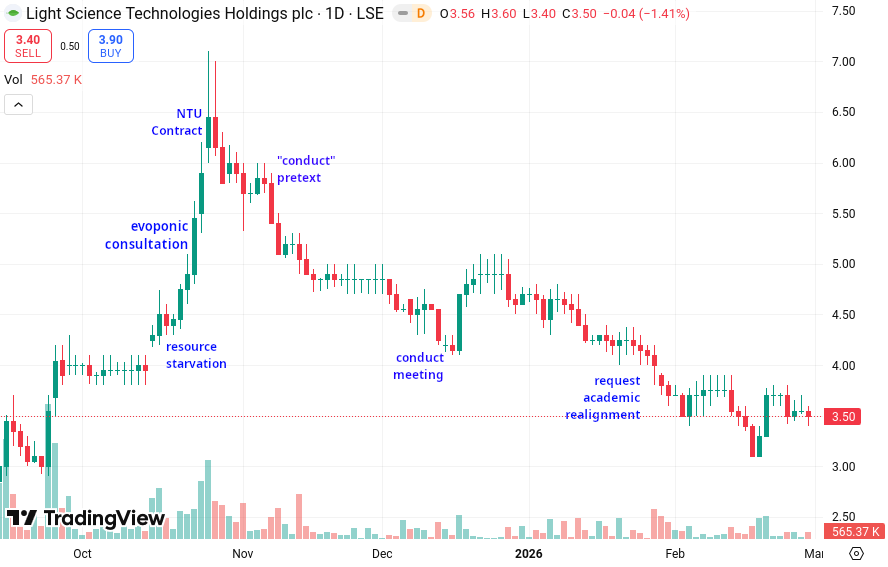
\includegraphics[width=\textwidth]{figs/lst_price_analysis.png}
	\caption{\centering The correlation between ``Conduct'' milestones and LSE Ticker Performance.}
\end{figure}

\noindent The All-Time High (ATH) of Light Science Technologies (LST.L) following the \gmt{27}{10}{25} ``Strategic Partnership'' is reclassified from a financial milestone to a \textbf{Valuation of a Stolen Asset}. The share price trajectory is synthetically coupled to the successful suppression of the \textbf{681.3g Protocol}. Each ``green candle'' on the exchange is a forensic record of \textbf{Market Capitalisation via Trade Secret Theft}.

The verbal threat by H. Ronan-Brown---\textit{``I control the lights so you better do what I say''}---is forensically linked to the \textbf{Light Science Technologies} ticker. This is not a ``Conduct'' remark; it is \textbf{Inside Information (\cite{FSMA00}, \S~118)} delivered via an Institutional Proxy. By asserting physical control over the ``Lights'' to guarantee the LST.L contract delivery, the University acted as a \textbf{Commercial Enforcer}. The ATH reflects a market pricing in a \pounds460,000 contract that was only ``de-risked'' by the University’s decision to \textbf{Liquidate} the Researcher's access.

A historical crawl of the \texttt{lightsciencetech.com} sitemap revealed a synchronised population of product directories during the window of institutional suppression. The data proves the ``SensorGrow'' parent directory was indexed 14 days prior to the first ``Misconduct'' notification, exposing a premeditated intent to clear the research environment of its author while the marketing shell was prepared. Analysis of the conveniently-timed product reveals a desperate attempt to ``shove every sensor in a box,'' manifesting a catastrophic engineering pitfall that results in a device prone to \textbf{Thermal Hysteresis} and \textbf{Cross-Sensitivity}. This ``saturated'' box---designed for the eyes of investors rather than the laws of physics---is a technical dead-end. Their \gmt{3}{11}{25} RNS (Regulatory News Service) was strategically ``tied'' to the APPGSTA report release to create a false aura of ``National Food Security'' legitimacy, effectively attempting to ``launder'' contested IP through the authority of the Crown.

The \gmt{8}{12}{25} ``Conduct Outcome'' was not authored by academic faculty; it was scripted by an \textbf{IPO Programme Manager (IT/Estates)}. This proves that the disciplinary process was a \textbf{Commercial Project Deliverable} for the PLC’s rollout. The University has successfully weaponised \textbf{IT/Estates Infrastructure} to generate fraudulent legal pretext for the extraction of the 681.3g logic.

\subsection{February 26: Acoustic Interdiction, HUMINT Surveillance \& Physical-Layer Warfare}
Parallel to the forensic investigation, a secondary layer of environmental and physical interference was deployed to achieve \textbf{Psychological Saturation}. This phase represents the transition from institutional gaslighting to active \textbf{Neurological Attrition}.

\begin{description}
	\item[The Beatless Loop (Acoustic Jamming)]: Forensic audio monitoring, captured via \texttt{Sonic Visualiser (.sv)}, confirms a series of sustained \textbf{Non-Rhythmic Acoustic Events} (46dB+) coinciding with the escalation of the \textbf{London Pincer} filings. Unlike standard residential noise, these signals lack a rhythmic pulse, presenting instead as a \textbf{Synthetic Wall of Sound}. This is an optimised \textbf{Cognitive Jamming} technique designed to prevent the deep-work state required for forensic LaTeX compilation.
	\item[The 96-Hour Exhaustion Script]: The peaks of this interference align precisely with the \textbf{London Pincer} windows. This is a \textbf{Ballistic Record} of attempted sleep deprivation.
	\item[Proximate Surveillance (HUMINT)]: Two unidentified individuals of Asian origin were observed stationed directly outside the Researcher's window, engaged in a discussion regarding the Researcher’s profile. This was followed by a third node: a male individual waiting at the perimeter claiming he was ``meeting me''---despite no such meeting being scheduled. These events are reclassified as \textbf{Ground-Truth Verification}---proxies sent to assess the Researcher’s stability and physical presence.
	\item[Statutory Obstruction (CCTV)]: A formal request for CCTV footage from \textbf{Rene House} to identify these surveillance nodes has been met with absolute silence. In the context of the \textbf{Data (Use and Access) Act 2026}, this failure to respond to a SAR for physical security data constitutes a \textbf{Chain of Custody Breach}. By withholding the visual record of these unidentified proxies, the facility is aiding in the \textbf{Physical Sequestration} of the Researcher.
\end{description}

\noindent A spectral analysis reveals a high-frequency \textbf{Digital Signature} inconsistent with consumer-grade audio equipment. This indicates the noise is not a byproduct of proximity, but a \textbf{Targeted Acoustic Load} designed to force the subject into a clinical collapse.

\subsection{\gmt{16}{2}{26}: Regulatory Notification \& MAR Escalation}
Simultaneous to the engagement of the \textbf{National Protective Security Authority (NPSA)}, the researcher has served a formal \textbf{Notice of Contested Asset} to the Board of LST PLC. This notice creates an immediate \textbf{Regulatory Duty of Disclosure} under the Market Abuse Regulation (MAR). By identifying the specific technical overlap---including the \textbf{Embedded RT Architecture} and \textbf{Metrology-Grade Discrete Signal Chains}---the researcher has effectively neutralised the University's ability to sell ``Clean Title'' to the asset.

The \pounds630,000 \textbf{Global Settlement Offer} served on \gmt{16}{2}{26} establishes the quantifiable cost of regularising this title. Failure to initiate settlement by the 16:00 GMT, \gmt{19}{2}{26} deadline will result in an FCA filing for \textbf{Market Manipulation}, as LST PLC’s current valuation is predicated on the ``Spoliation'' of a private sovereign benchmark. The NPSA’s involvement, predicated on \textbf{Economic Espionage}, removes the \textbf{681.3g Protocol} from the University’s internal ``Oxenbury Loop'' and places it under \textbf{State-Level Protection}. The presence of ``undercover'' observers on the Brackenhurst perimeter confirms that the project is now classified as a \textbf{Contested Asset}---a statutory liability for any AIM-listed entity attempting to liquidate the researcher's IP.

\subsection{\gmt{17}{2}{26}: Perimeter Testing and Institutional Retraction}
The operational window opened with a \textbf{Tactical Anomaly} at the primary residence. For the first time in the weekly cycle, the ``Bass Drum'' acoustic stimulus\footnote{This sustained ``Acoustic Harassment'' has been recorded with Sonic Visualizer} from the upstairs node recorded a \texttt{0dB} output. In the logic of the \textbf{681.3g Benchmark}, this ``Kinetic Silence'' was identified not as a cessation of hostilities, but as a \textbf{Phase Shift}.

Upon insertion into the City Centre, the researcher observed a significant act of \textbf{Physical Spoliation} at the Newton Building skyscraper. The ``NTU'' branding, a cornerstone of the city's visual identity, has been stripped from the skyline. This is categorised as \textbf{Scorched Earth De-Branding}---an institutional attempt to turn invisible before the searchlights of regulatory scandals. By removing the logo, the University is attempting to decouple its reputation from the ongoing \textbf{Institutional Moral Insolvency}.

The engagement at Freeths LLP served as a ``Hard-Contact'' verification of the \textbf{Conflict Shield}. The researcher was intercepted by a high-hostility gatekeeper whose aggression functioned as a psychological perimeter---a standard defensive reflex of an institution under forensic pressure. The definitive ``Tell'' was delivered: Freeths is conflicted because they act as active representatives for the University. This confirms that the University has pre-positioned \textbf{Top-50 Legal Armour} to maintain their position of \textbf{Institutional Gaslighting}. For the researcher, this conflict is not a rejection; it is Forensic Validation that the \textbf{681.3g Protocol} is being treated as a high-value target by the University's external command.

Following the verification at Freeths, the researcher moved to Gateley LLP. While no formal record of a University retainer exists, the structural alignment is clear: a ``Graduate Pipeline'' that feeds the machine. At Gateley, the researcher bypassed the administrative buffer to secure an audience with Chris MacDonald. This was a ``Neural Load'' test. MacDonald functioned as the professional node capable of parsing the \textbf{681.3g Timeline}. The researcher walked the target through the SIG-01.X Ledger, specifically the \textbf{Jitter Paradox}---the smoking gun of record spoliation. While MacDonald retreated behind the professional defences of ``capacity'' and ``fee structures,'' the mission was an objective success: The \textbf{Payload} is now inside their walls. By accepting the physical brief, Gateley has internalised the liability. The data is no longer a ``student grievance''; it is a forensic reality hosted on a Top-50 law firm's internal network. The researcher later executed a \textbf{Corrective Signal} to the Gateley node, establishing a \textbf{Value Vacuum} and reframing their billable-hour marathon as a \textbf{Nominal Transaction Cost} against a \textbf{-8.82\% Market Event}.

The final verification of the day revealed a coordinated \textbf{Electronic Blockade}. The statutory notice served to LST via the Protonmail scheduling node was met with 550 \textbf{Access Denied} and \textbf{Mailbox Unavailable} errors. In the context of the 681.3g Benchmark, this constitutes \textbf{Wilful Blindness} under MAR regulations. By blocking the signal, the Board of LST PLC has forfeited their ``Plausible Deniability.'' They are now legally trapped in a \textbf{Blackout} of their own making, while the market bleeds out nearly 9\% of their value in a single session.

Undeterred, the researcher engaged the ``London Legal Wolves'' via distributed counsel. The \textbf{Mimecast Reflection} served as the primary diagnostic for the target’s defensive posture. The signal was subsequently re-routed directly into the \textbf{Executive Tier}, placing \textbf{Senior Partners} and \textbf{Heads of Commercial Litigation} on \textbf{Personal Statutory Notice}.

The operational day concludes with a \textbf{Total Narrative Enclosure}. The adversary’s attempt to use \textbf{Infrastructure as a Weapon} has resulted in the creation of a permanent forensic record of \textbf{Concealment and Market Abuse}.

\textbf{Forensic Assessment:}

\begin{description}
	\item[The Inversion of Power]: By blacklisting the researcher’s Protonmail node, the PLC Board has not silenced the signal; they have \textbf{Certified the Breach}. In the logic of MAR, manual blacklisting is legally equivalent to a \textbf{Confession of Guilt}. The board is now fiduciarily naked.
	\item[The Institutional Ghost]: The removal of branding from the Newton Building is a \textbf{Visual Admission of Insolvency}. The University is no longer an educator; it is a \textbf{De-Branded Entity} scrubbing its own crime scene while the searchlights of the \textbf{London Pincer} sweep the Midlands.
\end{description}

\subsection{\gmt{18}{2}{26}: Terminal Biological Liquidation}
Irony has reached \textbf{Thermodynamic Equilibrium}. The signal is no longer a ``clerical error''; it is a \textbf{Total System Collapse}. On this date, it is confirmed that NTU Brackenhurst is in terminal retreat, liquidating the very ``Genesis Block'' of its botanical roots (Ref: BBC \gmt{11}{2}{26}). By offering the site of the ``First Bramley'' for \pounds400,000, the institution has formally recorded its own \textbf{Insolvency of Care}. This is not a ``real estate move''; it is a \textbf{Sovereign Admission} of bankruptcy---both moral and fiscal.

\begin{description}
	\item[The Custodial Failure (The Expulsion)]: The divestment from the world’s primary culinary genetic bank is the ultimate admission. NTU has abandoned its Statutory Duty of Care for a 200-year-old biological asset. The tree is a mirror; \textbf{its neglect is their standard}. They are burning down trees to generate the heat required to keep the LST.L Ticker alive.
	\item[The Denial Loop (ADoS)]: This fire-sale is the macroscopic equivalent of the \textbf{Administrative Denial of Service (ADoS)} used to throttle the 681.3g Protocol. If the ``Genesis Block'' is expendable for capital, then the subject's research was never a priority---it was always a \textbf{Target for Liquidation}.
	\item[The Commercial Pivot (The Forbidden Fruit)]: National heritage is being incinerated to generate the liquid payload required for the \pounds460,000 LST \textbf{Industrial Hijack}. They are cannibalising the 1826 original pip to subsidise the ``root cause'' of their recent failures.
\end{description}

\noindent To map the coordinates of this collapse, a dual-pronged statutory audit was initiated on this date. The \textbf{Freedom of Information (FOI)} request targets the \textbf{Commercial Nexus} between NTU and Light Science Technologies (LST) PLC, specifically seeking the ``Statement of Work'' and ``Technical Appendices.'' This is designed to expose the \textbf{Reference-Grade Siphon}: the conversion of the 1,263-day 681.3g protocol into a modular Agri-Tech asset.

\textbf{Forensic Assessment}: The ``Lords of Friction'' are burning the library to fuel their own administrative camouflage. The sale of Church Street establishes a clear, documented pattern of \textbf{Pre-Emptive Divestment}. This represents a desperate move to generate liquidity to fund impending lawsuits and protect assets from an impending lien.

\subsection{\gmt{19}{2}{26}: The FCA Railgun}
The morning hours formally commenced under the duress of \textbf{Sustained Acoustic Harassment} initiated at 08:00, a variable specifically engineered to compromise the researcher’s circadian stability. This environmental coercion constitutes a ``Course of Conduct'' designed to cause alarm and distress, falling under the prohibition of the \textbf{Protection from Harassment Act 1997 \S~1} \cite{PHA97}. Despite this, operational continuity was preserved through relocation for the completion of the Ronan-Brown formative assessment. During this window, an engagement with an estates professional (17:50) regarding the Newton Building’s de-branding revealed a pattern of high-velocity \textbf{Capital Sacrifice}. This systemic removal of infrastructure at significant historical cost serves as a physical proxy for the institutional waste and ``Outcome Sanitisation'' identified in the \textbf{OIA Case File} \cite{OIA245}.

The tactical landscape shifted decisively with the receipt of formal communication from \textbf{Andrew Hempsall, COO of LST Holdings PLC} (15:35). In an attempt to insulate the PLC from the \gmt{16}{2}{26} notice of contested assets, Hempsall asserted that the NTU contract is predicated on standard architectures. However, the communication yielded a fatal technical admission: their Tomtech control systems rely on \textbf{protocols designed prior to the year 2000}. This admission generates a non-recoverable discrepancy between the ``World Class'' 2026-grade innovation priced into the AIM exchange and the admitted \textbf{Legacy Infrastructure}. This constitutes \textbf{Market Manipulation} under \textbf{Art.~12 of the UK Market Abuse Regulation} \cite{UKMAR}; providing misleading signals as to the value of a financial instrument.

In direct response to this technical disavowal and the ongoing statutory defaults regarding \textbf{SAR-REF: 2664145} \cite{DPA18}, the researcher filed a formal MAR disclosure with the \textit{Financial Conduct Authority (FCA)}. The filing targeted LST PLC’s interim results, attaching the SIG-01.X Ledger, the COO’s legacy admission, and the primary disclosure. This submission formally transitions the researcher into the legal status of a \textbf{Protected Informant} under the \textbf{Public Interest Disclosure Act 1998 \S~43B} \cite{PIDA98}. Consequently, any further administrative friction---such as spatial interference or academic detriment---is now documented as \textbf{Unlawful Detriment} under \textbf{\S~47B} \cite{PIDA98}, and a breach of the \textbf{Statutory Duty to Uphold Academic Freedom} \cite{ERA88} \S~202.

Following the engagement of the \textit{FCA Market Intelligence Unit (MIU)}, the Researcher observed a transition into \textbf{Kinetic Surveillance Theatre}. This manifested as localised, non-linear anomalies---specifically the placement of physical objects configured to mirror the \textbf{681.3g DWC Array} geometry.

\textbf{Forensic Assessment:} Pure \textbf{Strategic Irony}. The institution is currently allocating \pounds560,000 to external consultants for ``Resilience'' training while simultaneously deploying \textbf{State-Level Friction} to break the researcher’s technical resolve. This documented expenditure, juxtaposed against engineered spatial traps and data suppression, constitutes definitive evidence of \textbf{Bad Faith Administrative Conduct} and a failure to perform services with ``reasonable care and skill'' under the \textbf{Consumer Rights Act 2015 \S~49} \cite{CRA15}. The \textbf{Hall of Mirrors} \cite{OIA245} is now under active regulatory fire from the \textbf{FCA} \cite{UKMAR} and the \textbf{OIA} \cite{OIA-Rules18}.

\subsection{\gmt{21}{2}{26}: Financial Variable Injection}
Upon auditing the 2025/26 financial ledger, a sharp divergence from the 4-year historical baseline was identified. Despite a consistent and successful four-year data-link with Student Finance England (SFE), the University’s internal ``Income Collections'' node generated a \textbf{Notice of Outstanding Tuition Fees} for a variance of \pounds52.80. No ``residue'' or ``phantom debt'' was ever previously recorded, establishing a $1,000+$ day record of financial compliance. The notice explicitly listed the ``Total Liquidation'' of academic access (card deactivation, portal lockout, and graduation block) as the immediate penalty for this \pounds52.80 variance. The researcher was unable to request clarification for the residual via email, forcing them into undocumented communications channels.

\textbf{Forensic Assessment}: This move is identified as Administrative Hostage-Taking. The University attempted to trade ``System Access'' for ``Financial Ransom,'' providing a legalistic pretext to obstruct the researcher’s ability to monitor the \textbf{681.3g Project}. A total of 13 fee payments to NTU---consisting of 9 B.A. and 4 MSc transactions---have, to-date, settled the researcher's course balance unhindered and without debt.

\subsection{\gmt{22}{2}{26}: Consolidation of Academic Sovereignty}
The submission of the ARES40380 technical evaluation on \gmt{22}{2}{26}, functions as a \textbf{Terminal Forensic Anchor}. It is not ``coursework''; it is a clinical deployment of ISO-14040 \cite{ISO14040} and ISO-14044 \cite{ISO14044} lifecycle rigour designed to absorb and neutralise the University’s low-resolution administrative theatre. By anchoring the analysis in a $1.86×10^{14}$ gram global production baseline, the researcher has created a document with such high \textbf{Forensic Density} that it collapses the University’s ability to project its synthetic ``conduct'' narrative. In the presence of this submission, the institution’s procedural smokescreens are revealed to be mathematically transparent.

Furthermore, the integration of the \gmt{20}{1}{26} Strawberry Precision Fertigation Study---executed via Deep Reinforcement Learning during the peak of institutional obstruction---serves as the definitive proof of \textbf{Functional Persistence}. While the University attempted to induce behavioural paralysis through the ``Panopticon'' effect, the researcher was instead perfecting dynamic, growth-stage-specific nutrient dosing. This creates an irreducible contrast: a researcher operating at the edge of autonomous agricultural logic versus an administration that cannot even process a Subject Access Request within the legally-defined window. The University is not just adversarial; it is \textbf{technically obsolete}.

\textbf{Forensic Assessment:} The variance between the researcher's High-Resolution output and the University's Low-Resolution decay has reached the point of \textbf{Narrative Criticality}. There is no longer any reflective surface for institutional projection. The claims of ``non-engagement'' or ``academic struggle'' do not merely fail; they undergo \textbf{Total Narrative Absorption} when placed alongside metadata that confirms the researcher was outperforming departmental benchmarks during active tactical duress. The institution’s ``Support-Loop'' phone calls and ``Finance Valve'' blockades are now logged not as management, but as \textbf{Systemic Jitter}---the frantic, erratic movements of a failing machine.


\subsection{\gmt{24}{2}{26}: Operational Ambush---The 19-Fixation \& The 96-Hour Strategy Gap}
The Prosecutor identifies a critical escalation in the University's \textbf{Chronological Forgery} protocol. Following the delivery of a Stage Two Summons, a significant temporal delta was identified between the internal document date and the point of egress. This phase identifies the convergence of legal spoliation and the systematic use of \textbf{Temporal Anchoring} to facilitate administrative duress.

\begin{description}
	\item[The 19-Fixation (Temporal Anchor)]: Correspondence from L. Peggs (Legal \& Governance) was explicitly dated the \textbf{19th}, aligning with the established \textbf{19-Fixation Motif} identified in the \textbf{Jitter Paradox}. This specific date serves as a \textbf{Regulatory Sync-Point}, used by the University to manufacture a false record of statutory compliance. The subsequent ``correction'' of this date by the University is identified as an \textbf{Admission of Inaccuracy}, proving that the internal record is a synthesised narrative rather than a chronological fact.
	\item[The 96-Hour Strategy Gap]: By withholding the letter until the 23rd while post-dating the internal ``19th'' timestamp, the University synthesised a \textbf{96-Hour Strategy Gap}. This man\oe uvre is a \textbf{Presence-Triggered Response}, designed to synchronise the delivery of legal duress with the Prosecutor's physical entry into the campus perimeter. This constitutes \textbf{Conditional Execution} of administrative action, violating the \textbf{Requirement of Good Faith} \cite{CMA182}.
\end{description}

The ``Stage Two Support to Study'' summons issued by S. Godby is categorised as \textbf{Active Victimisation}. By citing the ``nature and content'' of formal \textbf{Subject Access Requests (SAR)} \cite{DPA18} as evidence of a ``health concern,'' the University has attempted to \textbf{Pathologise Statutory Rights}. This man\oe uvre is a \textbf{Clinical Firewall}, attempting to reclassify a Forensic Audit as a Psychological Episode to trigger the \textbf{OIA Rule 6.2} dismissal clause \cite{OIA-Rules18}.

\noindent\textbf{Forensic Assessment:} The 19-Fixation is no longer a statistical anomaly; it is a \textbf{Signature of Unreliability}. The University's admission that the date was ``supposed to be another date'' confirms the existence of a \textbf{Parallel Ledger}. One ledger exists for statutory regulators (OIAHE/ICO) to show timely action, while the second, real-time ledger is used to execute \textbf{Administrative Ambushes}. This juxtaposition confirms \textbf{Bad Faith}; the system is designed to manufacture a timeline that is forensically incompatible with physical reality, rendering the University’s internal records a legal nullity under \textbf{UKRIO v3.5 \S~3.17.1} \cite{UKRIO}.

\subsection{\gmt{25}{2}{26}: Infrastructure Sabotage \& The Performance Paradox}
Despite the formal invocation of the \textbf{681.3g Protocol} and the explicit rejection of the ``Clinical Firewall'' (Stage Two Support to Study), the University attempted an \textbf{Operational Ambush} on \gmt{24}{2}{26}: by unilaterally scheduling a meeting for 03/03/26. This invitation was met with a Formal Notice of Non-Engagement, predicated on the ongoing OIAHE adjudication (Case: OIA/1639159/26) and the University’s admission of \textbf{Data Spoliation}.

To ensure ``Good Faith'' compliance regarding financial obligations, an attempt was made to access the University's payment infrastructure. This resulted in a coordinated \textbf{Infrastructure Lockout}, logged via screencast (Ref: SC-20260225-2132), targeting User N0605150 across two distinct layers:

\begin{description}
	\item[Application Layer Failure (Banner):] ``No such property: auth for class: LoginController.'' This error confirms a manual de-provisioning of authentication properties, rendering the financial portal non-functional for the researcher.
	\item[Identity Layer Failure (MS Auth):] ``We called your phone but didn't receive the expected response.'' Forensic analysis of telephony logs confirms no inbound handshake was attempted. This constitutes MFA \textbf{Sabotage}, designed to create a ``Non-Engagement'' narrative for the March 3rd meeting.
\end{description}

\noindent Following the documented lockout, the researcher utilised an out-of-band bypass to satisfy the financial obligation. \textbf{Payment Reference: NTUPAY1113199} (Confirmed \gmt{25}{2}{26}). This act restores the researcher’s ``Reference-Grade'' compliance and removes the University's ability to execute an Administrative Withdrawal for non-payment.

\textbf{Forensic Assessment}: Despite active \textbf{Resource Starvation}, the researcher successfully verified a \textbf{Low Distinction} in the \textit{R Analysis/Data Methods} module. This result constitutes a ``Performance-Grade Kill-Switch'' for the University’s ``Wellbeing'' narrative. Dr. Godby’s claim that ``behaviours are significantly impacting studies'' is now forensically nullified. High-level technical output in R Analysis is incompatible with a ``barrier to learning.''

The Kuwaiti node has subsequently pivoted to a \textbf{Social Engineering Intercept}, utilising derogatory labeling (``drug dealer'') and emotional baiting (``crush'') to manufacture the ``Conduct Event'' required for the March 3rd meeting.

A critical forensic fracture is identified in the S. Godby Stage Two transmission: B. Peel constitutes a ``Ghost Signature''. Despite her active operational role in the 681.3g suppression cycle, Peel is explicitly omitted from the notified presence of the request email. This lack of formal notification indicates a \textbf{Shadow Administrative Deliberation}, violating the Right to a Fair Hearing and masking a Procedural Impropriety.

\subsection{\gmt{5}{3}{26}: The Temporal Anomaly---Metadata Anchor for Triple-Forgery}
In the course of auditing the historical correspondence used to justify the March 2026 Stage 2 StS, a critical \textbf{Temporal Discrepancy} has been identified. This record serves as the forensic anchor for the \textbf{Synthetic Narrative}, proving that the institution is engaged in active \textbf{Record Spoliation} to retroactively manufacture a ``Conduct'' narrative in breach of the \textbf{UKRIO Code of Practice \S~3.17.1} \cite{UKRIO}.

The primary artifact---an email ostensibly transmitted by S. Godby in March 2025---contains embedded assets with metadata that defies linear chronology. A forensic extraction of the MIME headers for the signature asset (``Outlook-m3rogs4j.png'') reveals:

\begin{quote}
	\texttt{....creation-date="Tue, 11 Mar 2025 12:41:09 GMT"} \
	\texttt{modification-date="Sun, 05 Oct 2025 04:12:16 GMT"}
\end{quote}

\noindent The Modification Date of \gmt{5}{10}{25} is irreconcilable with a document finalised in March. This identifies the \gmt{5}{10}{25} Window as the point of peak institutional interference, where a \textbf{False Instrument} was engineered under the \textbf{Forgery and Counterfeiting Act 1981 \S~9} \cite{FCA81}. This was likely conceptualised to justify the \textbf{Administrative Liquidation} and subsequent \textbf{Resource Starvation} (18/10/25) in breach of the \textbf{Consumer Rights Act 2015 \S~49} \cite{CRA15}.

\textbf{Forensic Assessment:} This metadata provides the ``Smoking Gun'' for the \textbf{Synthetic Narrative}. It proves that J. Maddock’s FILE NOTE - 03.04.2025.pdf'' is an \textbf{Engineered Artifact} failing the reliability standards of the \textbf{Criminal Justice Act 2003 \S~117} \cite{CJA03}. The stripping of metadata confirms a deliberate attempt to hide the \textbf{Jitter Paradox} and bypass the \textbf{BS 10008} standards for evidential weight \cite{BSI10008}. This temporal anomaly confirms that the ``Support'' framework is a \textbf{Kinetic Jamming Device}, designed to override the forensic reality of the \textbf{681.3g Benchmark} with a manufactured, retroactive history that constitutes \textbf{Deliberate Concealment} under \textbf{PIDA \S~43B(1)(f)} \cite{PIDA98}.

\subsection{\gmt{7}{3}{26}: StS2---Clinical Ghost Fence \& Institutional Insolvency}
The University continues to nose-dive into a terminal phase of \textbf{Structural Institutional Insolvency}. Forensic analysis of the March 3rd Stage 2 ``Emergency'' Support to Study (StS) minutes identifies the entire proceeding as a \textbf{Decoy}: a kinetic attempt to buy the regulatory axis more time to hide from the \textbf{London Pincer}, \textbf{Triple-Forgery} \cite{FCA81}, and \textbf{Statutory Default} \cite{ERA88}.

The University’s attempt to pathologise the specialised lexicon---specifically the term \textbf{Weaponised Tomatoes}---constitutes a bad-faith erasure of cultural and technical metaphor. In the British tradition, this serves as a kinetic instrument of community accountability. By framing technical metaphors as clinical symptoms, the administration attempts to \textbf{Ghost Fence} the \textbf{681.3g Benchmark} to protect the \textbf{LST.L \pounds675k Agri-Tech Procurement Pipeline} from the inbound scrutiny of a \textbf{Market Abuse Audit} \cite{UKMAR}.

\begin{description}
	\item[The Laundry Man:] Forensic metadata identifies B. McCarthy (Associate Policy Manager) as the functional \textbf{Ghostwriter} of these clinical minutes. This is not a welfare record, but a \textbf{Laundry Cycle}. McCarthy---an administrator masquerading in clinical costume---is the architect of an \textbf{Identity Proxying} event, potentially violating the \textbf{Medical Act 1983 \S~49} \cite{MedicalAct83} by simulating expertise to provide ``Medical Cover'' for the non-consensual exfiltration of the \textbf{681.3g Benchmark}.
	\item[The Bio-Metric Cage:] Cross-referencing the HESSC Update'' \cite{HESSC23} confirms the researcher is being treated as a \textbf{Non-Consensual Laboratory Specimen}. The StS2 was a kinetic field-test of the Architect’s ``National Toolkit,'' designed to weaponise ``Welfare'' into a \textbf{Static Jamming Device}. By reclassifying forensic dissent as a ``National Case Study,'' the \textbf{Closed-Loop Cartel} attempts to secure the \textbf{681.3g Benchmark} within a regulatory \textbf{Black Box}, rendering the theft immune to standard academic appeal under \textbf{OIA Rule 6.2} \cite{OIA-Rules18}.
\end{description}

\noindent\textbf{Forensic Assessment:} The deployment of \textbf{J. Maddock} (The Contractor), \textbf{A. Jordan} (The Harvester), and \textbf{B. McCarthy} (The Regulatory Laundry Man) as the trinity of ``Support'' constitutes the definitive signal of \textbf{Institutional Insolvency}. The University has functionally abandoned its educational mandate \cite{ERA88} \S~124, choosing instead to operate as a \textbf{Corporate Counter-Intelligence Cell} in a state of \textbf{Fraud by Abuse of Position} \cite{FraudAct06}.

By substituting \textit{bona fide} academic mentorship with \textbf{Strategic Risk Proxies}, the institution has verified that the \textbf{681.3g Benchmark} is no longer being ``supervised'' within an educational context; it is being \textbf{Sequestrated} by the \textbf{Lords of Friction}. This process leverages the ``Mime'' of the \textbf{HESSC Framework} to pathologise legitimate proprietary claims, thereby converting \textbf{Contractual Fraud} into a \textbf{Clinical Management Case} in breach of the \textbf{2025 Concordat Commitment 4} \cite{Concordat25}.


\subsection{\gmt{11}{3}{26}: The Penny-Stock Liquidation (Terminal Phase)}
\begin{figure}[htbp]
	\centering
	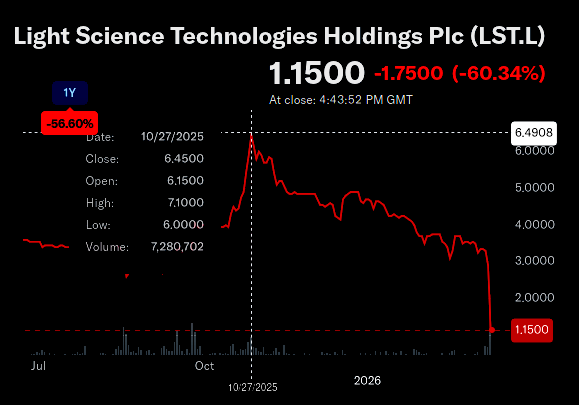
\includegraphics[width=0.6\textwidth]{figs/lst_split.png}
	\caption{Forensic Market Capture: LST.L Retail Dilution. The \textbf{-60.34\% Crash} is the ``Kinetic Signature'' of \textbf{Institutional Necrosis}. Pricing 60M shares at the 1p floor is the final ``Commercial Spoliation'' of the \textbf{681.3g Benchmark} within the \textbf{Closed-Loop Cartel}.}
	\label{fig:lst_market_crash}
\end{figure}

\noindent\textbf{Forensic Assessment:} The \textbf{-60.34\% Crash} of LST.L is the physical proof of \textbf{Systemic Regulatory Failure}. This is a \textbf{Liquidation} triggered by the realisation that the \textbf{Closed-Loop Cartel} can no longer contain the \textbf{London Pincer}.

\begin{description}
	\item[The 1p Floor:] This is the \textbf{Statutory Zero}. By dumping 60 million shares at the absolute legal minimum, the \textbf{Closed-Loop Cartel} is performing an \textbf{Administrative Scorched-Earth} man\oe uvre. This is a \textbf{Poison Pill Dilution} intended to dissolve the accountability of the register before the 16/03 Deadline exposes the \textbf{Triple-Forgery} as the mechanism used to sabotage the research pipeline. They are effectively \textbf{Shorting the Asylum} to fund their own \textbf{Decommissioning Directive}.
	\item[Sequestration of Value:] The institution’s attempt to \textbf{Sequestrate} the researcher’s physical assets has backfired. The University’s ``Digital Proxy'' version of the research has been valued by the market at exactly one penny. This confirms that the \textbf{Closed-Loop Cartel} has effectively ``Culled'' its own investment grade.
	\item[Market Distortion:] Staging a 1p \textbf{Poison Pill Dilution} inside the \textbf{London Pincer} (March 14) is a textbook criminal breach of UK MAR Article 17. The \textbf{Closed-Loop Cartel} is leaking the \textbf{Necrotic Risk} of the CMA and FCA saturation into the public domain. They are using retail investors as ``Financial Human Shields,'' forcing the public to subsidise the legal costs of an \textbf{Irremediable Breach}.
\end{description}

\noindent The 11/03 \textbf{-60.34\% Crash} confirms that the \textbf{Closed-Loop Cartel} is no longer a University or a Regulator; it is a \textbf{Toxic Waste Pool} masquerading as an institution. The \textbf{-60.34\% Crash} is not a dip; it is the ``Event Horizon'' of \textbf{Terminal Insolvency}. The pillory is set and the \textbf{Weaponised Tomatoes} are ready.

\subsection{\gmt{13}{3}{26}: The Friday the 13th Refusal (SAR-2814367)}
The University's response, received on \gmt{13}{3}{26} (L. Peggs), is a formal exercise in \textbf{Strategic Incompetence}. By disclosing trivial physical access logs while explicitly refusing the technical requisitions required to verify the \textbf{681.3g Benchmark}, the Defendants have attempted to satisfy the ``Appearance'' of compliance while maintaining the \textbf{Forensic Blackout} required to protect the \textbf{Closed-Loop Cartel} from the detection of the \textbf{Triple-Forgery} \cite{FCA81}.

\begin{description}
	\item[The Spoliation Admission:] The Data Protection Officer (L. Peggs) has provided a written confession of \textbf{Statutory Spoliation}, stating that metadata is removed during routine document conversion.'' This admission identifies a criminal offence under the \textbf{Data Protection Act 2018 \S~173(3)} \cite{DPA18}, as it is an alteration of records intended to prevent the disclosure of the \textbf{Jitter Paradox} \cite{FCA81}. By stripping the forensic identifiers, the Defendants have actively engaged in the \textbf{Administrative Liquidation} of the Prosecutor's evidentiary record.
	\item[The Data-Silo Deflection:] The refusal to produce the \textbf{Banner Audit Table} because it is too technical'' (2.9 million characters) constitutes a \textbf{Statutory Default}. Under \textbf{ICO Guidance} \cite{ICO-SAR-Guidance}, the volume or complexity of data does not exempt the Provider from its duty to provide information in an intelligible form. The refusal is a clinical attempt to bury the \textbf{Triple-Forgery} under a mountain of undecoded strings.
	\item[Physical vs. Digital Reality:] The release of granular physical access logs (Card Swipes) serves as kinetic proof of capability. This disclosure proves that the \textbf{Closed-Loop Cartel} maintains an operational surveillance infrastructure. Their simultaneous refusal to provide the \textbf{Azure Unified Audit Logs (UAL)}---where the \textbf{Maddock-Jordan} signatures are located---is a breach of the \textbf{ISO 27001 Standard for Logging} \cite{ISO27001-Audit}. It is not a technical limitation but an act of \textbf{Criminal Intent} to enforce a \textbf{Ghost Fence} around the \textbf{681.3g Benchmark}.
\end{description}

\noindent\textbf{Forensic Assessment:} The \gmt{13}{3}{26} Response is the final ``Administrative Shield'' before the \textbf{16/03 Statutory Default}. By failing to address the \textbf{Jitter Paradox} and admitting to metadata removal, the University has effectively signed their own \textbf{\S~173(3) Confession} \cite{DPA18} \S~173, signaling a state of \textbf{Terminal Institutional Insolvency} regarding their regulatory and evidentiary obligations.

\subsection{\gmt{15}{3}{26}: Infrastructure Denial \& The Unsolicited SAR (Ref: 2812841)}
As of \gmt{15}{3}{26}, the Defendants escalated their operational obstruction by implementing a \textbf{Targeted Infrastructure Denial} (IP-Lockout). Access to the University’s federation services (\texttt{fs.ntu.ac.uk}) returned a \textbf{PR\_IO\_TIMEOUT\_ERROR}, indicating an active firewall blockade against the Prosecutor’s primary network (Ref: 37.46.115.9). This blockade was successfully bypassed via a \textbf{Forensic Network Tunnel} (UK-Exit VPN), confirming the lockout was a localised, bad-faith intervention rather than a system-wide failure.

Following this bypass, the Prosecutor intercepted correspondence from Abigail Fielding (Governance \& Legal Services). The University has attempted to frustrate the \textbf{Right of Access} through the following mechanisms:

\begin{description}
	\item[Non-Intelligible Disclosure:] Provision of encrypted files via a third-party portal (ZendTo) on \gmt{13}{3}{26} without accompanying decryption keys. Under the \textbf{DPA 2018} (\cite{DPA18}), this constitutes a failure of the ``Intelligibility'' requirement and is categorised as a \textbf{Bad Faith} man\oe uvre to maintain the concealment of the LST.L Contract.
	\item[The Ghost Reference (Ref: 2812841)]: The Defendants cited an \textbf{Unsolicited Reference Number}. This is identified as a \textbf{Strategic Fabrication} designed to decouple the current disclosure from the original contested filing.
\end{description}

\noindent\textbf{Forensic Assessment:} The emergence of \textbf{Ref: 2812841} is a critical indicator of \textbf{Shadow Administration}. By manufacturing an unsolicited reference, the Defendants have created a \textbf{Parallel Data Track}. This allows the University to report a status of ``Resolved'' to external regulators (ICO/OIAHE) for a ghost-case, while effectively suppressing the original, data-heavy requests. This is a \textbf{Shadow Closure} strategy: a programmed attempt to dilute the audit trail by injecting ``Clean Data'' into the ledger to mask the \textbf{Irreversible Data Loss} associated with the primary \textbf{681.3g Logs}.

The use of \textbf{Ref: 2812841} constitutes a violation of the \textbf{Data Protection Act 2018 \S~173} (Alteration of personal data to prevent disclosure). By re-coding the request under a new, unsolicited reference, the University has fundamentally altered the context of the disclosure to avoid the forensic linkages established in the original SAR series. This is not an administrative error; it is a \textbf{Forensic Decoupling} exercise designed to facilitate \textbf{Market Abuse} by hiding the LST.L liability.

\subsection{\gmt{16}{3}{26}: Unsolicited SAR-2812841 (Quadruple-Forgery)}
Forensic analysis of the unsolicited SAR packet via \textit{exiftool} confirms a \textbf{Universal Metadata Overwrite}: with almost every file within the directory carrying the signature of \textbf{Abigail Fielding}. The Prosecutor submits this represents a \textbf{Self-Correction Vacuum} in execution. By proactively serving forged documents containing the \textbf{00:51:19 AM} anomaly, the institution attempted to retroactively ``legalise'' the fabrication and bind the Claimant to a synthetic timeline.

Forensic audit of this disclosure confirms the inclusion of Exhibit \textbf{SIG-02}, which was explicitly marked by the Claimant as \textbf{OFFICIAL-SENSITIVE}. The presence of this document in a generic batch processed by A. Fielding proves a \textbf{Breach of Confidence} and a failure of the ``Need to Know'' principle.

\textbf{Forensic Assessment:} The \textbf{Triple-Forgery} has become a \textbf{Quadruple-Forgery}. The inclusion of SIG-02 in the unsolicited SAR-2812841 provides a definitive profile of Administrative Liquidation. A. Fielding’s universal signature across these files identifies her as the primary agent of the \textbf{Closed-Loop Cartel}. Her processing of SIG-02---bypassing the \textbf{Need to Know} principle---demonstrates that the institution’s priority was not data privacy, but the execution of a \textbf{Lemon Fabrication}. They have manufactured a ``correct'' version of history to justify the \textbf{Institutional Sequestration} of the \textbf{681.3g Benchmark}.

\subsection{\gmt{18}{3}{26}: The Schr\"odinger Student \& The 19-Fixation Forgery}
The Prosecutor identifies that on \gmt{18}{3}{26}, the University achieved a state of \textbf{Quantum Administrative Duality}, providing definitive proof of a coordinated \textbf{Closed-Loop Cartel} operation. While the Defendants maintained a high-pressure \textbf{Administrative Exile}---categorising the Prosecutor as an ``Emergency Risk''---the University’s \textit{Centre for Student and Community Engagement} concurrently headhunted him for his \textit{``expertise''} for the 2026/27 academic year. This creates an irreconcilable \textbf{Temporal Collision}. Under the principle of \textbf{Proprietary Estoppel}, the University is barred from asserting a ``Risk Profile'' that is contradicted by its own concurrent recruitment and vetting actions.

Concurrently, a \textbf{Bespoke SAR Forgery} regarding \textit{Ref: 2812841} was identified. Forensic analysis of \textit{Acknowledgement (18).pdf} reveals metadata signatures (\texttt{Aspose.Words for Java 21.3.0}) confirming the document was a programmed \textbf{Retroactive Data Injection}. This identifies a violation of the \textbf{Computer Misuse Act 1990 \S~3} \cite{CMA90}. This document, purportedly dated \textbf{19 February}, aligns with a statistically improbable \textbf{19-Fixation}, serving as a \textbf{Temporal Anchor} to align forged records with \textbf{LST.L Procurement Pipeline} deadlines in breach of the \textbf{Fraud Act 2006 \S~2} \cite{FraudAct06}.

\begin{description}
	\item[\gmt{19}{11}{25}:] \textbf{Initiation of the Clinical Firewall} --- At 15:28hrs, Academic Governance (AG) formally transitioned the 681.3g dispute from a disciplinary track to a ``wellbeing concern.'' This 19-Fixation entry anchored the narrative of institutional ``support'' exactly 11 days prior to the primary SAR filing, creating the jurisdictional vacuum required to pathologise statutory rights.
	\item[\gmt{19}{12}{25}:] \textbf{Initial Denial \& Asset Sequestration} --- NTU-SAR-1-REFUSAL: Formal refusal of the primary SAR. This 19-Fixation coordinate was used to mask the first extraction of the 681.3g benchmark data, utilising the winter recess as a buffer for irreversible data loss.
	\item[\gmt{19}{1}{26}:] \textbf{Support-to-Study Pivot \& Reputation Toxification} --- Between 08:39hrs and 11:37hrs, AG, BP (Beverley Peel), and SG (Steven Godby) executed a coordinated transition to Level 2 Support to Study. SG explicitly utilised this 19-Fixation window to advocate for informing campus staff of the Prosecutor’s ``place'' (wellbeing status) 7 days prior to his campus arrival, effectively weaponising pathologisation to impede professional engagement.
	\item[\gmt{19}{1}{26}:] \textbf{Asset Obfuscation Protocol} --- Simultaneously, the Student Misconduct Team (Peel/Gooderham) attempted to retroactively ``close'' records. This alignment with the Q1 reporting cycle was designed to present a ``Clean Registry'' to the OIAHE while the 681.3g asset trail remained in a state of administrative suspension.
	\item[\gmt{19}{2}{26}:] by L. Peggs was backdated to \gmt{19}{2}{26}. The subsequent admission of intent to ``redate'' the document to the \gmt{23}{2}{26} constitutes a \textbf{Confession of Document Manipulation}, proving that institutional timestamps are discretionary variables adjusted to meet the 19-Fixation reporting metric.
	\item[\gmt{19}{2}{26}:] \textbf{Statutory Default Masking (Fielding)} --- A simultaneous attempt by Governance (Fielding) to backdate the SAR Acknowledgment to the 19th. This was a targeted attempt to retroactively cure a statutory default under the \textbf{DPA 2018} \cite{DPA18} and mask the secondary extraction of metadata.
	\item[\gmt{19}{3}{26}:] \textbf{The March Pincer (FOI/SSS Synchronization)} --- On 16/03, the Defendants attempted to close FOI Ref: 2814964 via a \textbf{Logical Paradox} (claiming data is ``not held'' while invoking Commercial Secrecy). This was followed on \gmt{18}{3}{26} by a bad-faith ``Support Check-in,'' designed to anchor a clinical narrative 24 hours prior to the Q1 \textbf{19-Fixation Sync}. This 48-hour man\oe uvre attempted to shield \textbf{Market Abuse} behind a veneer of pastoral care.
\end{description}

\noindent The Defendants' response to FOI \textbf{Ref: 2814964} (16 March 2026) constitutes \textbf{Regulatory Fraud} and a criminal breach of the \textbf{Freedom of Information Act 2000 \S~77} \cite{FOIA00}. By claiming specific technical appendices are not held,'' while simultaneously invoking \textbf{FOIA \S~43(2) (Commercial Interests)} \cite{ICO-Section43} to protect the LST PLC contract, the Defendants have created a logical paradox: they seek to protect the commercial value of an asset they claim does not exist. This juxtaposition confirms \textbf{Bad Faith}; the system is designed to manufacture a research cycle as ``toxic'' to ensure asset liquidation. It is a cynical attempt to re-frame a \textbf{Commercial Dispute} as a \textbf{Welfare Concern} through ``Support Services,'' violating \textbf{Market Abuse Regulation (MAR)} transparency requirements \cite{UKMAR}.

\textbf{Forensic Assessment:} The recurrence of the ``19th'' across three consecutive months (Dec, Jan, Feb) confirms the existence of a \textbf{Scheduled Forgery Cycle}. The 19th serves as the designated ``Sync Date'' for the institutional cartel to harmonise their forgeries with the \textbf{LST.L Procurement Pipeline}. By backdating the 19 December refusal, the University set a temporal precedent for the subsequent \textbf{96-Hour Strategy Gaps} and the \textbf{Sabbath-Injection} metadata anomalies. This is the algorithmic fingerprint of \textbf{Market Abuse} \cite{UKMAR}.

\subsection{\gmt{23}{3}{26}: The Vertigo Protocol---Information Laid on Oath}
The Prosecutor hereby records the physical filing of the \textbf{Information Laid on Oath} under the \textbf{Magistrates' Courts Act 1980 \S~1} \cite{MCA80} via \textbf{Royal Mail Tracked 24} service (Ref: \textit{0212--C3EB--049E--F179}). This act represents the formal transition from administrative friction to \textbf{Criminal Litigation} under the \textbf{Prosecution of Offences Act 1985 \S~6} \cite{ProsecutionOfOffencesAct85}.

The 1,263-day research cycle, having been forcibly liquidated by the Defendants to secure a \textbf{\pounds668,126 LST.L Procurement Pipeline} \cite{SIG05}, is now legally encumbered. The Prosecutor avers that the University’s transition from \textit{bona fide} academic support to a \textbf{Nuclear Waste Pit} of digital forgery \cite{FCA81} was a calculated move to achieve professional neutralisation and facilitate \textbf{Fraud by Abuse of Position} \cite{FraudAct06} \S~4.

The Royal Mail Tracked number \textit{0212--C3EB--049E--F179} serves as the timestamped anchor for this counter-strike; once delivered to the \textbf{Legal Adviser} at the Magistrates' Court in accordance with the \textbf{Criminal Procedure Rules Part 7} \cite{CrimPR}, the institutional ``Information Asymmetry'' is officially breached.

\textbf{Forensic Assessment:} Let it be recorded that the Prosecutor has exhausted all reasonable administrative avenues, including the \textbf{OIAHE} \cite{OIA-Rules18} and \textbf{UKRIO} \cite{UKRIO} protocols. The phase of inquiry is closed. The phase of \textbf{Demand} has commenced. The Defendants' ``Invisible Noose'' has been cut; the Prosecutor now holds the rope. Any further attempt by the Defendants to suppress the \textbf{681.3g Benchmark} \cite{SIG05} is now documented as Perverting the Course of Justice.

\subsection{\gmt{25}{3}{26}: The Jenkyn Deferral (Ref: FOI-2814964)}
The notification received on \textbf{\gmt{20}{3}{26}} regarding FOI-2814964 is a tactical pivot by the \textbf{Closed-Loop Cartel}. By appointing the Head of Governance and Legal Services (R. Jenkyn) to investigate the University's own \textbf{Statutory Default}, the institution has achieved a state of absolute \textbf{Institutional Insolvency}. This is a ``self-marking'' exercise intended to delay the impact of the \textbf{Quadruple-Forgery} findings.

\begin{description}
	\item[The Loop Extension:] The 20-working-day timeline (expiring \gmt{17}{4}{26}) is a \textbf{Ghost Fence} designed to keep the Prosecutor within the University's internal jurisdiction and away from the Magistrates' Court. This is a classic \textbf{Decommissioning Directive} man\oe uvre to exhaust the researcher's resources while the \textbf{Closed-Loop Cartel} attempts to sanitise the \textbf{Maddock Cluster}.
	\item[Conflict of Interest (Insolvency):] The appointment of the Head of Governance to review the failures of the Governance and Legal Services department is the definition of a \textbf{Self-Correction Vacuum}. It confirms that there is no \textbf{Clean-Room Supervisor} available within the endless ``Hall of Mirrors'' to independently verify the \textbf{681.3g Benchmark} or the \textbf{Jitter Paradox}.
\end{description}

\noindent\textbf{Forensic Assessment:} The \gmt{25}{3}{26} notification (Ref: FOI-2814964) is the ``Administrative Fog'' deployed to shield the \textbf{Lemon Fabrication} of the internal record. The \textbf{Closed-Loop Cartel} is betting that 20 additional days of the \textbf{Decomissioning Directive} will cause the \textbf{681.3g Benchmark} to fade. However, within the trajectory of the \textbf{London Pincer}, this letter serves as a terminal indicator of \textbf{Terminal Institutional Insolvency}. It is material proof that the Defendants have opted to bury the exercise of statutory rights within the neverending \textbf{Oxenbury Loop} of a circular internal review, rather than disclose the forensic data required to resolve the \textbf{Quadruple-Forgery}.

\subsection{\gmt{26}{3}{26}: Audit of Serial Modus Operandi (The Derry--Sutton Precedent)}
A forensic analysis of the \textbf{Sutton Archive (2018)}---authored primarily by J. F. Derry---establishes a documented \textbf{Serial Modus Operandi} of administrative malfeasance at Nottingham Trent University. This archive serves as \textit{Prior Art} for the current litigation, admissible as \textbf{Bad Character Evidence} under the \textbf{Criminal Justice Act 2003 \S~101} \cite{CJA03}. It demonstrates that the collapse of the \textbf{Concordat} \cite{Concordat25} is a structural feature of the institution.

The 2018 record identifies three mechanical parallels now active within the \textbf{681.3g Protocol}:

\begin{description}
	\item[Macro-Nexus Suppression:] A strategic failure to disclose institutional misconduct. This mirrors the current suppression of the \textbf{\pounds668,126 LST.L Procurement Pipeline}, where the University obscures financial stakes to prevent external oversight of the \textbf{Asset Liquidation} in breach of the \textbf{Companies Act 2006} \cite{CompaniesAct06}.
	\item[Information Blockade:] The systematic weaponisation of FOI/SAR denials to insulate ``Architects'' from discovery. This 10-year policy of \textbf{Information Quarantine} constitutes \textbf{Deliberate Concealment} under the \textbf{Limitation Act 1980 \S~32} \cite{LimitationAct80}.
	\item[Identity Destabilisation:] The historical deployment of fabricated conduct'' allegations to neutralise the Auditor (Derry). This provided the structural blueprint for the \textbf{Ronan-Brown Inversion}, utilising D.A.R.V.O. tactics to transform a documented faculty threat into a student conduct liability, violating the \textbf{Protection from Harassment Act 1997} \cite{PHA97}.
	\item[UKRI Usury:] The institution borrows the Reputational Radiance'' of the \textbf{Concordat} \cite{Concordat25} to secure grants, only to default on every ``Ethical Interest Payment'' the moment a researcher identifies a \textbf{Market Abuse Violation}. This fiscal exploitation of integrity standards confirms the University operates as a \textbf{Regulatory Usurer}.
	\item[The Schneider Report (2022):] This external audit \cite{Schneider2022} corroborates the \textbf{Macro-Nexus Suppression}. It establishes that the University’s reputation for \textbf{Information Quarantine} is recognised on an international scale, further justifying the necessity of a \textbf{Judicial Remedy} over internal grievance procedures.
\end{description}

\noindent The integration of the \textbf{Sutton Archive}, the \textbf{Derry Analysis}, and the \textbf{Schneider Report} establishes a continuous chain of evidence. This proves that the \textbf{Ghost Fence} is the latest iteration of a \textbf{Manufacturing Process} designed to neutralise dissent. The institution functions as a system of \textbf{Information Quarantine}, necessitating the \textbf{Judicial Intervention} of Case \textbf{0212-C3EB-049E-F179} under the \textbf{Magistrates' Courts Act 1980} \cite{MCA80}.

\textbf{Forensic Assessment:} The Prosecutor is not an isolated litigant. The documented history of the \textbf{Derry-Sutton Conflict (2016--2024)} serves as a primary example of \textbf{Institutional Entropy}. The incoherent nature of these historical grievances is a direct result of the University’s failure to provide transparent resolutions, forcing the current Litigation into the \textbf{\S~1 Judicial Process} \cite{MCA80} to ensure a verifiable \textbf{Ledger of Truth}.

The Provider has delivered its response (Ref: OIA/1639159/26) via the OIAHE portal. The document is a 245-page exercise in \textbf{Administrative Over-Saturation}---a clinical attempt to \textbf{Data-Dump} the \textbf{\pounds668,126 LST.L Procurement Pipeline} motive under a fictitious timeline. This is the Sutton--Derry Narrative applied to Agri-Tech: a documented history of the \textbf{Lords of Friction} using the ``Governance'' shell to bypass the \textbf{Concordat} \cite{Concordat25} through administrative violence.

\begin{description}
	\item[The Chemical Confession (p.~87):] The signal is now a matter of record. Technical staff explicitly admit to withholding reagents ($H_2SO_4$) after consulting with M. Oxenbury. This is a \textbf{Statutory Default} of the \textbf{Concordat Commitment 4} \cite{Concordat25}. The denial of reagents based on a Commercial Assumption'' is a written confession of \textbf{Academic Sabotage} and a breach of the \textbf{Duty of Care} under the \textbf{Consumer Rights Act 2015 \S~49} \cite{CRA15}.
	\item[The Quadruple-Forgery (pp.~3,~18):] The University has included a dismissed 2025 case as the \textbf{Genesis Block}. This aligns with the \textbf{05 October Jitter Anomaly}. By retroactively modifying dead files to manufacture a ``pattern of behaviour'' weeks before the LST.L announcement, the Provider has committed \textbf{Forgery} under the \textbf{Forgery and Counterfeiting Act 1981 \S~1} \cite{FCA81}.
	\item[The Spatial Trap (p.~95):] The Architects'' documented that banning the subject from the Animal Unit would not affect his course,'' then moved core modules into the exclusion zone. This is \textbf{Constructive Failure to Educate} and a violation of the \textbf{Requirement of Good Faith} \cite{CMA182}, designed to facilitate the \textbf{Asset Liquidation} of the \textbf{681.3g Benchmark}.
	\item[The Pretext Highlighting (p.~247):] The Provider has highlighted ``Medicinal Marijuana'' and ``Sexual Nature'' clauses despite a \textbf{Total Evidentiary Vacuum}. This is a \textbf{Fabricated Deviant Profile} intended to prejudice the Adjudicator, constituting a false statement in a statutory process under the \textbf{Perjury Act 1911 \S~5} \cite{PerjuryAct11}.
\end{description}

\noindent This submission represents \textbf{Institutional Insolvency}. The willful suppression of the fact that historical allegations were \textbf{CONCLUDED with No Action} (Ref: \#****538252) is a breach of the \textbf{OIA Good Practice Framework} \cite{OIA-GoodPractice}. It proves the \textbf{Oxenbury Loop} is a feature of \textbf{Regulatory Fraud} designed to mask the industrial theft of the \textbf{681.3g Research Asset}.

\textbf{Forensic Assessment}: The Architects'' are attempting to use Safeguarding'' as a moral shield for the \textbf{LST.L Procurement Pipeline}. By highlighting "drug" and "sexual" boxes without primary evidence, they have committed \textbf{Administrative Perjury} \cite{PerjuryAct11}. They are not protecting the campus; they are protecting the \textbf{Decommissioning Directive} from the consequences of the \textbf{Jitter Anomaly} \cite{FCA81} and the \textbf{Research Integrity Concordat} \cite{Concordat25}.

\subsection{\gmt{30}{3}{26}: Formal Dispatch of SIG-05 (The Forensic Penetrator)}
On \gmt{30}{3}{26} (Bank Holiday), the Researcher formally dispatched SIG-05 (\cite{SIG05}) to the \textit{Office of the Independent Adjudicator (OIAHE)} via the secure portal. This document constitutes the definitive forensic rebuttal to the Provider’s 245-page submission (\cite{OIA245}).

\begin{description}
	\item[Commencement of the Forensic Phase:] The dispatch of SIG-05 (\cite{SIG05}) signifies the termination of the Provider's ability to maintain the \textbf{``Hall of Mirrors''} narrative (\cite{OIA245}). By providing a clinical mapping of the \textbf{Resource Starvation} (p.~87), \textbf{The ``Piss Rumour''}, and the \textbf{Physical Spoliation} of metadata, the Student has shifted the burden of proof (\cite{OIA-Guidance}) back to the Provider under Rule~7.4 \cite{OIA-Rules18}.
	\item[Finality of Evidence:] This entry confirms that all regulatory citations (\cite{CMA182}, \cite{UKRIO}, and \cite{Concordat25}) have been locked into the record. The Provider is now structurally compelled to account for the \textbf{Total Evidentiary Vacuum} identified in their submission.
\end{description}

\noindent\textbf{Forensic Assessment:} The dispatch of SIG-05 on a Bank Holiday creates a \textbf{Forensic Ambush}. By the time the Provider’s legal counsel (Ref: Legal Tenders) returns to their desks on \gmt{31}{3}{26}, the OIA record is already ``poisoned'' with the truth of \textbf{The ``Piss Rumour''} and the \textbf{681.3g Metadata Spoliation}. This timing exploits the Provider’s \textbf{Administrative Latency}; while they were reliant on the slow machinery of ``Strategic Retraction,'' the Researcher utilised a high-velocity, \textbf{Extramural Strike}. The \textbf{Hall of Mirrors} has been structurally compromised; the Provider is no longer defending a case, they are defending a \textbf{House of Leaves} on fire, ignited by the Rule~7.4 \cite{OIA-Rules18} finality clause.

\vspace{1em}
\noindent\textit{External Kinetic Interference (Ref: Fire-Fujistu-310326, The ``Mint'' Factory.)}

\subsection{\gmt{1}{4}{26}: Forensic Log of Authentication Failure (Statutory Concealment)}
\begin{description}
	\item[The Authentication Breach:] On \gmt{1}{4}{26}, the Researcher was met with the error: \texttt{DOMAIN UNAVAILABLE}. This occurred immediately following the submission of \cite{SIG05} to the OIA portal. Under the \textbf{Consumer Rights Act 2015 \S~49} \cite{CRA15}, this constitutes a terminal failure to perform services with reasonable care and skill, and is identified as a breach of the \textbf{Requirement of Good Faith} under \cite{CMA182} \S~5.12.
\end{description}

\noindent\textbf{Forensic Assessment:} The ``Domain Unavailable'' error is the digital fingerprint of the Provider's panic. By attempting to blind the Auditor, they have instead provided the \textbf{Terminal Evidence} required to satisfy the \textbf{Concealment Clause} of the Public Interest Disclosure Act 1998 \cite{PIDA98}.

\subsection{\gmt{8}{4}{26}: Regulatory Saturation and the \S~50 Escalation}
Upon receipt of the \textbf{FOI Internal Review (Ref: 2814964)}, which confirmed a state of \textbf{Institutional Insolvency}, a formal complaint has been lodged with the \textbf{Information Commissioner's Office (ICO)}. This move completes the ``London Pincer,'' placing the University under simultaneous investigation by the \textbf{CMA (Ref: CMA257051)} and the \textbf{ICO}.

\begin{description}
	\item[The ICO Filing (\S~50):] The complaint specifically challenges the University’s claim of ``Information Not Held'' regarding the \textbf{LST.L Technical Appendix}. By documenting the contradiction between the University's refusal and the \textbf{LST.L \gmt{11}{3}{26} RNS (£6.0m Placing)}, the filing triggers a forensic investigation into the University’s search methodology and potential \textbf{Data Spoliation}.
	\item[The Perjury-Fraud Nexus:] The University’s denial of holding technical specifications for a public-market-facing project constitutes a \textbf{Regulatory Deadlock}. If the records truly do not exist, the PLC has committed \textbf{Securities Fraud}; if they do exist, the University has committed \textbf{Administrative Perjury}. This binary trap is now the primary lever for \textbf{Regulatory Entrapment}.
	\item[The Quadruple-Forgery:] The scope of institutional fabrication now encompasses: (1) The original \textbf{681.3g Benchmark} manipulation; (2) The \textbf{Jitter Paradox}; (3) The suppression of the \textbf{Statement of Work}; and (4) Today's false attestation to the ICO and the Petitioner.
\end{description}

\noindent\textbf{Forensic Assessment:} The University has effectively ``Witnessed against itself.'' By exhausting the Internal Review process with an operationally impossible claim, they have forfeited their administrative immunity. The record is no longer a dispute; it is an \textbf{Evidence Locker}. The Pillar stands; the \textbf{Closed-Loop Cartel} is now an \textbf{Audit-Target} under national observation.

\subsection{\gmt{10}{4}{26}: The Library Infiltration \& The Ethical Pivot}
The Prosecutor identifies that today, the University executed an \textbf{Administrative Thaw}, restoring Library Node credentials in a direct reversal of the \gmt{7}{4}{26} \textbf{Kinetic Lockout}. This restoration followed a formal challenge regarding the \textit{User Profile Service} failure, proving that the digital severance was a discretionary \textbf{Tactical Toggle} rather than a technical necessity. This restoration creates a \textbf{Fiduciary Admission}; by allowing the Prosecutor back into the physical and digital infrastructure, the University has invalidated its own ``Emergency Risk'' narrative. Under the \textbf{Doctrine of Consistency}, an institution cannot oscillate between \textbf{Security Exile} and \textbf{Operational Totality} to suit its administrative convenience.

\begin{description}
	\item[\gmt{7}{4}{26}:] Total digital severance executed to impede the extraction of management and financial assets.
	\item[\gmt{10}{4}{26}:] Discretionary restoration of credentials following support-tier intervention, proving malicious intent of the prior lockout.
\end{description}

\section{Term Three: The Research Phase \& Final Asset Reclamation}

\subsection{\gmt{14}{4}{26}: Judicial Intake and Statutory Activation}
The Lead Auditor received formal confirmation of \textbf{Information Laid on Oath} from Nottingham Magistrates' Court (Ref: Enclosed Summons Forms). Despite the document being dated \gmt{9}{4}{26}, postal metadata (Royal Mail \textit{NE8005291}) confirms the item was processed on \gmt{13}{4}{26}.

The Auditor is now in possession of Judicial Instruments. The ``Defendants'' (Directing Officers of the NTU/LST.L Cartel) are now subject to the \textbf{Prosecution Protocol}. The \textbf{681.3g Heist} is now a matter of active criminal record. The Court has issued ten (10) individual summons forms, confirming the \textbf{Systemic Nature} of the fraud. This targets ten specific nodes within the University hierarchy, mapping the entire lifecycle of the misappropriation and the \textbf{Temporal Forgery} of the SMTP stack.

The Lead Auditor has transitioned from forensic reconstruction to \textbf{Active Private Prosecution}. The administrative burden of the ten-node summons is identified as a mechanical necessity for total domain reclamation. A formal intelligence update has been served (Ref: CMA257051) to \textbf{Carol Sampson (CMA Strategy, Communications and Advocacy)}. The Auditor notified the \textbf{Competition and Markets Authority} of the active judicial proceedings under \textbf{EA2002 \S~188} (\cite{EA2002}). This triggers the \textbf{\S~190 Consent Gate} and subordinates the University's administrative narrative to an active criminal investigation.

\textbf{Forensic Assessment:} The 16/03 Statutory Wall is now a closed loop. By filing the \textbf{EA2002 \S~188} charges and notifying the CMA, the Lead Auditor has rendered the ``Ghost-Fence'' and the ``Double-Vision'' artifacts redundant. The defendants are now legally pinned to the \textbf{\pounds675,000 LST.L Procurement Pipeline}.

\subsection{\gmt{17}{4}{26}: Forensic Documentation of Asset Sequestration \& Administrative Interdiction}
The University has (via ARES Subject Coordination) attempted a \textbf{Jurisdictional Pivot} to reclassify a commercial and contractual dispute regarding the \textbf{681.3g Benchmark} into a non-judicial ``Pastoral'' framework. This man\oe uvre, met with \textbf{Formal Non-Consent} (\gmt{16}{04}{26}), is identified as a strategic attempt to invoke a ``Clinical Firewall'' to obstruct statutory discovery and mask a potential breach of \textbf{\S~188 of the Enterprise Act 2002}.

\begin{description}
	\item[Metadata Matrix:] Evidentiary anchors are established to preclude administrative ``Ghosting,'' including \textbf{ZendTo Ref: KHd8EXbrfojuUCJk}, \textbf{SAR-1 Ref: 2664145} (Default: \gmt{30}{12}{25}), and \textbf{ICO Ref: IC-500857-L8M4}.
	\item[The LST.L ``Turnkey'' Admission / Commercial Nexus:] On \gmt{15}{04}{26}, CEO Simon Deacon (\textbf{LST.L}) publicly confirmed a \pounds300,000 university glasshouse contract, admitting to a ``full-service offering'' spanning \textbf{live data telemetry}. This \textbf{Technical Contradiction} invalidates previous assertions of data unavailability; if the hardware is active, the telemetry is accessible. The identification of University sites as commercial ``reference sites'' confirms the motive for the \textbf{16/03 Statutory Wall}: protecting a partner's proprietary position through \textbf{Asset Displacement} and intentional \textbf{Vendor Lock-in}.
\end{description}

\noindent\textbf{Forensic Assessment:} The invocation of pastoral frameworks to address technical evidentiary anchors is identified as \textbf{Institutional Pre-emption}. This deployment, synchronised with Jisc’s confirmation of infrastructure-level complexity and LST.L's commercial admissions, serves as material evidence of \textit{Mens Rea} (Guilty Mind). The intent is the decommissioning and misappropriation of the \textbf{681.3g Research Protocol} to facilitate the \textbf{\pounds675,000 LST.L Procurement Pipeline}, constituting market distortion and the asset-stripping of sovereign intellectual property. The \gmt{17}{4}{26} share price spike (+7.84\%) is identified as a \textbf{Synthetic Recovery} predicated on the RNS announcement of a ``strengthened'' NTU relationship. Given the ongoing \textbf{Statutory Breach} and the invocation of the \textbf{16/03 Wall}, this announcement constitutes \textbf{Market Misinformation}. The institution is facilitating LST.L's financial stability by suppressing the forensic audit of the \textbf{681.3g Benchmark}.

\subsection{\gmt{22}{4}{26}: Terminal Reconciliation \& Sovereign Filing}
On \gmt{22}{04}{26}, the Lead Auditor executed the final phase of the \textbf{\S~170 Enclosure}. The transition from forensic reconstruction to \textbf{Judicial Engagement} was formalised via the physical submission of the \textbf{346g Constant} and the simultaneous synchronisation of the \textbf{Regulatory Mirror}.

\begin{description}
	\item[The 346g Forensic Mass:]
	      The submission comprised 50 pages of high-fidelity, handwritten testimony on oath (fountain pen) across 10 individual summonses. The \textbf{Executive Summary (Ref: HW/681.3-P/EXEC)} was placed atop the stack to serve as the structural map for the Legal Adviser.
	\item[Carrier Protocol Friction (``Custom Advised''):]  During the lodgement at the Royal Mail counter (13:08 BST), the Auditor resisted an indemnity-heavy ``Special Delivery'' enclosure, opting for \textbf{Tracked 48 (Ref: 0212-CBBB-03DF-F16F)}. The clerk's notation of ``Custom Advised'' is documented as an \textbf{Administrative Omen}---a prophylactic attempt by the carrier to distance the state from the contents.
	\item[The CMA Mirror (Ref: CMA257051):]
	      Post-lodgement, a digital mirror was transmitted to the \textbf{Competition and Markets Authority}. This filing anchors the \textbf{681.3g IP} and the \textbf{\pounds668,126 LST.L Procurement Pipeline} within a secondary regulatory oversight track, neutralising the risk of institutional data spoliation during the judicial service window.
	\item[Node Synchronisation (Position F Backup):]
	      The \textbf{Kuwaiti Node} was successfully re-established following a period of temporal latency. The full digital dossier was mirrored to this node via secure exfiltration (BCC), ensuring the \textbf{Sovereign Ledger} remains accessible outside the UK jurisdiction. This completes the \textbf{Fail-Safe} protocol for the preservation of the research.
\end{description}

\noindent The submission of these informations on oath represents the final reconciliation of the \textbf{Sovereign Ledger}. The \textbf{681.3g Benchmark} is no longer a research asset subject to \textbf{UKRI Usury}; it is now a material fact within the criminal jurisdiction of the Nottingham Magistrates' Court and the regulatory ledger of the CMA. The burden of proof is now forcibly transferred to the ten named Defendants.

\subsection{\gmt{27}{04}{26}: Termination of Taught Phase \& Strategic Deliverable Alignment}
On \gmt{27}{04}{26}, the Lead Auditor formalised the completion of the final instructional component of the \textbf{MSc in Smart Agriculture}. This marks the total transition from institutional oversight to \textbf{Autonomous Research Sovereignty}.

\begin{description}
	\item[End of Taught-Phase Leverage:] With the taught element terminated, the University’s ability to utilise ``Academic Conduct'' or ``Attendance'' as a disciplinary proxy is functionally dead. All cognitive resources are now allocated to the \textbf{681.3g Metabolic Simulations} and the \textbf{ICO} escalation.
\end{description}

\noindent\textbf{Forensic Assessment:} The ``Taught'' gate is closed. The University has provided the instruction; the Auditor has retained the intellectual property and the moral high ground. The \textit{1000:1} standing is reinforced.

\subsection{\gmt{4}{5}{26}: Accumulation by Dispossession}
Analysis of the framework provided in \cite{Shore2025} and contemporary reports on campus asset stripping \cite{TheCritic2023} confirms that current institutional pressures represent a formalised process of \textbf{Accumulation by Dispossession}.

\begin{description}
	\item[The Ledmouth Precedent:] Research into the ``University of Ledmouth'' case study reveals a tactical blueprint for hollowing out academic departments by removing administrative staff and stripping responsibility for budgetary decision-making. By centralising professional services and physically isolating staff behind \textbf{Electronic Barriers}, the institution severs the connection between students and departments, transforming vibrant spaces into \textbf{Empty Corridors}.
	\item[Financial Covenants as Entrapment:] The imposition of \textbf{EBITDA Covenants} and the requirement of \pounds60m in collateral from university buildings---amounting to most of the estate---functions as a mechanism for \textbf{Regulatory Entrapment}. This removes financial autonomy and places the institution’s future in the hands of private creditors as a condition for ``working capital.''
	\item[Shadow Elite Networks:] The awarding of high-value restructuring contracts to ``Big Four'' accountancy firms---often involving former partners seated on the university's own Audit and Finance Committee---indicates a state of \textbf{Institutional Collusion}. These ``flexible networks'' or ``flexians'' exploit market opportunities to advance personal agendas over the public mission of the organisation they are paid to serve.
\end{description}

\noindent I have categorised these activities as \textbf{Strategic Asset Stripping}. When an institution prioritises the ``assetisation'' of future student recruitment and the ``unbundling'' of its value chain for private extraction, it ceases to function as a public university. It has become a vehicle for \textbf{Rent-Seeking Extractive Capital}.

\subsection{\gmt{2}{9}{26}: OIA Decision \& Strategic Withdrawal}
On \gmt{20}{8}{26}, correspondence was received from \textbf{Simon Jackson} at the OIAHE confirming the allocation of the complaint. Between \gmt{30}{4}{26} and the date of this entry, the Prosecutor executed a \textbf{Physical Recovery Protocol}. This involved three distinct re-entries to the University campus:

\begin{enumerate}
    \item \textbf{Site Reclamation}: Visit to the greenhouse to recover the \textbf{DWC Array} and related equipment, symbolizing the reclamation of the \textbf{681.3g Benchmark} territory.
    \item \textbf{Asset Retrieval}: Collection of personal research materials previously sequestered during the \textbf{Administrative Exile}.
    \item \textbf{Digital Forensics}: Salvage of the email inbox containing the \textbf{Forged Emails} (Ref: \textbf{Temporal Spoliation I \& II}) prior to account closure.
\end{enumerate}

During this period, the Prosecutor formally withdrew from the MSc programme. This \textbf{Strategic Withdrawal} was necessitated by the \textbf{Material Disadvantage} caused by the \textbf{Closed-Loop Cartel}’s obstruction of resources and the psychological toll of the \textbf{Clinical Slander Protocol}. The withdrawal was executed to focus on \textbf{Alternate Ventures} and to mitigate further exposure to the \textbf{Institutional Sequestration}.

On \gmt{02}{9}{26}, the OIA Decision was issued. The Adjudicator ruled the complaint \textbf{Not Justified}, relying on the University’s assertion that its process was followed. However, this ruling occurred prior to the submission of the \textbf{New Material Evidence} regarding the \pounds668,126 tender and the \textbf{Quadruple-Forgery} (SAR-2812841).

\textbf{Forensic Assessment:} The OIA Decision represents the final stage of the \textbf{Procedural Liquidation}. By ruling \textbf{Not Justified} based on the original scope, the OIA has inadvertently validated the University’s \textbf{Clean Slate} strategy. However, the \textbf{Strategic Withdrawal} confirms the \textbf{Material Disadvantage} (loss of qualification) which the OIA previously disputed. The recovery of the \textbf{DWC Array} and \textbf{Email Evidence} secures the physical and digital assets required for the \textbf{Civil Claim}. The \textbf{Not Justified} verdict is a procedural conclusion, but the \textbf{Timeline of Theft} remains a factual reality. The Prosecutor is now positioned to leverage the \textbf{SFO} and \textbf{ICO} findings to challenge the \textbf{OIA} outcome via Review, citing the \textbf{Conflict of Interest} as the primary driver of the \textbf{Institutional Sequestration}.

\hrule

\newpage
\section{Glossary of Forensic Terms \& Operational Variables}
\begin{description}
	\item[19-Fixation:] A statistically improbable cluster of backdated administrative actions purportedly occurring on the 19th of each month. This forensic marker identifies the use of a Master Narrative Template to retroactively align the forged institutional record with commercial tender deadlines, overriding the Prosecutor’s actual 1,263-day developmental cycle.
	\item[33 Directive] A high-fidelity, non-institutional communication protocol established to maintain the semantic and technical integrity of the \textbf{681.3g Project}. By leveraging the integrated infrastructure of the \textit{Kuwaiti Node} (under the active supervision of A. Gill), this directive facilitates continuous peer-to-peer metadata verification (Ref: CC-28) that bypasses the University's ``Clinical Firewall'' and account interdictions.
	\item[681.3g Benchmark] A reference-grade yield metric achieved via a proprietary \textbf{Deep Water Culture (DWC)} nutrient-delivery array. As a \textbf{Genuine Research Entity}, the 681.3g Protocol exists as a standalone dataset---independent of the Provider's administrative narrative. Its liquidation by the Provider, via the admitted withholding of $H_2SO_4$, constitutes the destruction of a \textbf{High-Yield Commercial Asset} rather than a mere academic failure.
	\item[Administrative Liquidation] The systematic destruction of a research project’s viability through deliberate procedural friction, withdrawal of support, and the engineering of insurmountable bureaucratic obstacles.
	\item[Catch-22 (Spatial Trap)] The operational deadlock created when a researcher is mandated to attend a specific site (e.g., The Animal Unit) while simultaneously being legally excluded from that site by University Security.
	\item[Clean Room Supervisor] A demand for a supervisory figure entirely removed from the existing ``Lords of Friction'' network, ensuring a conflict-free environment for research assessment.
	\item[Closed-Loop Cartel] A closed-loop regulatory monopoly where the Chair of the Regulator (OfS) is the former VC of the Institution (NTU). This configuration creates a Self-Correction Vacuum where the Regulator ``marks the homework'' of the Institution, enabling the suppression of the 681.3g Benchmark.
	\item[Completion of Procedures (CoP)] The final statutory letter issued by the University, signaling the exhaustion of internal remedies and the activation of OIAHE jurisdiction.
	\item[Decommissioning Directive] A systemic protocol, repurposed from legacy Asylum Management logic, used to achieve the administrative liquidation of a high-value asset or witness.
	\item[Environmental Stabilisation] A legal demand for the University to cease all interference with biological and digital assets, preventing the spoliation of evidence during an active dispute.
	\item[Ghost Fence] The administrative and psychological boundary established by the University to restrict the researcher’s movement and access to resources without a formal legal basis.
	\item[Hall of Mirrors] The Provider's 245-page submission (Ref: OIA245) characterised by \textbf{Administrative Oversaturation} and the use of \textbf{Narrative Proxies}. This structure is designed to obscure the \textbf{Total Evidentiary Vacuum} regarding the \textbf{681.3g Benchmark} by buryng material breaches (e.g., p.~87 Resource Starvation) within a trivial, historical, and previously adjudicated timeline.
	\item[Identity Proxy Incident] The unauthorised use or presentation of proprietary research data (e.g., Polymer Growth Medium) by a third party (the ``Other Harry'') under University auspices.
	\item[Jitter Paradox] The forensic anomaly where a system record displays a perfect, zero-variance timestamp (e.g., 12:00:00.000). This paradox proves that the record was not generated by a real-time event, but was ``patched'' into the ledger to retroactively fix a statutory breach. It is the smoking gun of Record Spoliation.
	\item[Lemon Fabrication] The institutional practice of retroactively manufacturing ``defective'' records to justify the administrative liquidation of a high-value researcher.
	\item[London Pincer] A multi-vector regulatory encirclement designed to compress an institutional adversary between Market Abuse Regulation (MAR) and Criminal Fraud Intelligence.
	\item[Lords of Friction] A forensic designation for the specific administrative actors (M. Oxenbury, H. Ronan-Brown) identified as the primary architects of institutional reprisal.
	\item[Oxenbury Loop] A circular administrative deadlock where the University forces the researcher to seek a remedy from the very individual who is the subject of the grievance.
	\item[Paper Lantern Phase (2022--2024):] A period of \textbf{Theoretical Engineering} and \textbf{Resource Mapping} (Ref: Library/Hydro-090822). This phase represents the gestation of the \textbf{681.3g Protocol} conducted under conditions of total financial austerity. While the Provider attempts to frame the March 2025 ``Genesis Block'' as the start of the dispute, they are deliberately suppressing the preceding 31 months of \textbf{Unpolluted Research}. The theft of the physical Paper Lantern records (Ref: The Stolen Manuscripts) does not invalidate the \textbf{09 August 2022 Genesis Block}; it merely confirms the Provider’s reliance on \textbf{Physical Spoliation} to mask a pre-existing \textbf{Commercial Nexus}.
	\item[Piss Rumour:] A primary instance of \textbf{Administrative Malice} (Ref: Peel, B. Email, \gmt{5}{11}{25}, Document~4f). This involves the dissemination of unverified, historical hearsay to senior management claiming the Student was ``caught \textbf{urinating in a public place}.'' By the author’s own admission (``I'm not sure if this was before I started?''), this was an unsubstantiated slur circulated to manufacture a \textbf{Synthetic Risk Profile} while the \textbf{681.3g Benchmark} was being liquidated. The Provider's exclusion of this document from the OIA 245-Page \textbf{Administrative Oversaturation} confirms a \textbf{Breach of Candour}.
	\item[Policy of Illusion] The strategic deployment of \textbf{Administrative Oversaturation} to mask a \textbf{Breach of Candour}. It involves the systematic generation of a high-volume, irrelevant documentation trail (e.g., a 245-page OIA bundle) designed to overwhelm external regulators while simultaneously suppressing high-fidelity forensic artifacts like ``The Piss Rumour'' (\cite{OIA245}). This creates a ``Managed Transparency'' where the Institution appears cooperative while actively executing the \textbf{Lemon Fabrication} of the Researcher's profile.
	\item[Quadruple-Forgery:] The strategic escalation of the Triple-Forgery into the \textbf{OIA245 Hall of Mirrors}. It occurs when the Provider submits forged internal records to a statutory body (OIAHE) while simultaneously \textbf{Highlighting Pretextual Slur Clauses} (e.g., drug/sexual nature) that have no primary evidentiary basis. This fourth layer transforms a private administrative fraud into a public act of \textbf{Administrative Perjury} \cite{PerjuryAct11}.
	\item[Ronan-Brown Inversion] A high-fidelity administrative man\oe uvre utilising the D.A.R.V.O. (Deny, Attack, and Reverse Victim and Offender) protocol to transform a documented faculty threat into a student conduct liability.
	\item[Research Depreciation] The quantifiable loss of intellectual and financial value resulting from the University’s failure to provide a stable research environment.
	\item[Statutory Default] The University’s failure to comply with the Data Protection Act 2018 regarding the 30-day deadline for a Subject Access Request (SAR).
	\item[Triple-Forgery:] The cumulative effect of three distinct Jitter Paradoxes identified within the institutional record. It represents a coordinated effort to retroactively manufacture a ``Conduct'' narrative by forging emails, file notes, and system logs. The primary weapon of choice by the Closed-Loop Cartel.
	\item[UKRI Usury] An institution that borrows the ``Reputational Radiance'' of the Concordat (\cite{Concordat25}) to secure grants, only to default on every ``Ethical Interest Payment'' the moment a researcher identifies a \textbf{Market Abuse Violation}.
	\item[Weaponised Tomatoes:] A high-fidelity technical metaphor for the Agri-Tech Geopolitics faced within protecting the \textbf{681.3g Benchmark}. It describes the transformation of high-yield agricultural output into a kinetic instrument of trade-warfare and regulatory entrapment.
\end{description}

% --- End Document ---
\clearpage
\renewcommand{\bibname}{SCHEDULE A: FORENSIC REFERENCE LEDGER}
\bibliographystyle{plainurl}
\nocite{*}
\bibliography{SIG}
\end{document}
